\documentclass[UTF8, xcolor=table]{beamer}
\usepackage[BoldFont,SlantFont]{xeCJK}
\setCJKmainfont[BoldFont={Adobe Heiti Std},ItalicFont={Adobe Kaiti Std}]{AdobeSongStd-Light}
% \setCJKmainfont[BoldFont={Adobe Heiti Std},ItalicFont={Adobe Kaiti Std}]{SimSum} %Windows先编译使用这个字体

\usepackage{latexsym,amssymb,amsmath,amsbsy,amsopn,amstext,xcolor,multicol}
\usepackage{graphicx,wrapfig,fancybox}
\usepackage{pgf,pgfarrows,pgfnodes,pgfautomata,pgfheaps,pgfshade}
\usepackage{thubeamer}
\usepackage[backend=bibtex,sorting=none]{biblatex} % [参考文献格式](https://www.sharelatex.com/blog/2013/07/31/getting-started-with-biblatex.html) %mac IEEE not found
\usepackage{array}
\usepackage{bm}
\usepackage{caption}
\RequirePackage[font=footnotesize]{subcaption}
\usepackage{multirow}
\usepackage{booktabs}
\usepackage{tikz}
\usepackage{tikzscale}
\usepackage{animate}

\defbibheading{bibliography}[\bibname]{} %avoid printbibliography 自动生成目录
\addbibresource{../main.bib}
\setbeamertemplate{bibliography item}[text] 

\usepackage{boxedminipage} %for: bvh border
\def\fourgraphicswidth{0.35} %0.3\textwidth

\usepackage{algorithm} %%format of the algorithm
\usepackage{algpseudocode}
\floatname{algorithm}{算法}
\renewcommand{\algorithmicrequire}{\textbf{输入:}} % Use Input in the format of Algorithm
\renewcommand{\algorithmicensure}{\textbf{输出:}} % UseOutput in the format of Algorithm
\algrenewcommand{\algorithmiccomment}[1]{ $//$ #1}

\usepackage{listings}
\renewcommand\lstlistingname{代码}
\renewcommand\lstlistlistingname{代码}

\lstset{framexleftmargin=1.4em,
        xleftmargin=1.8em,
        basicstyle=\ttfamily\small,
        %frame=shadowbox, numberstyle=\tiny, breaklines=true,
        frame=single,
        numberstyle=\tiny, breaklines=true,
        keywordstyle=\color{blue!70}\bfseries,
        %commentstyle=\color{red!50!green!50!blue!50},
        rulesepcolor=\color{red!20!green!20!blue!20},
        numbers=none,fontadjust=true}
\lstdefinelanguage{shader}{morekeywords={uniform, layout, uniform, vec2, vec3, vec4, in, out, gl_Position, dot, flat, int ,float, gl_VertexID, xyz, w, x, y, z, location, version, sampler2DRect, bgr, gl_FragData, texture2DRect, gl_TexCoord,for,xy},morecomment=[l]{//}}

\begin{document}

\setbeamerfont{footnote}{size=\tiny}
\setbeamerfont{caption}{size=\scriptsize}
\setbeamertemplate{caption}[numbered]
\setbeamerfont{subsection in toc}{size=\footnotesize}
\renewcommand*{\bibfont}{\footnotesize}

\graphicspath{{../}}

\title[融合长短记忆神经网络与卷积特征学习的图像语义分割]{中山大学本科毕业论文演示文稿非正式模版}
\author[陈冠英]{}%{(申请中山大学工学学士学位论文答辩报告)\\ \vskip 20pt 学~~~~~~生:陈~冠~英}
\institute[中山大学~电子信息与工程学院~\&~自动化]{}%{\small \vskip 38pt 电子信息与工程学院~自动化}
\date{} %{\small \vskip -17pt二〇一六年五月}

%% make title %%
\frame{
	\titlepage
	\vspace{-23mm}
	\begin{figure}[h]
		\centering
		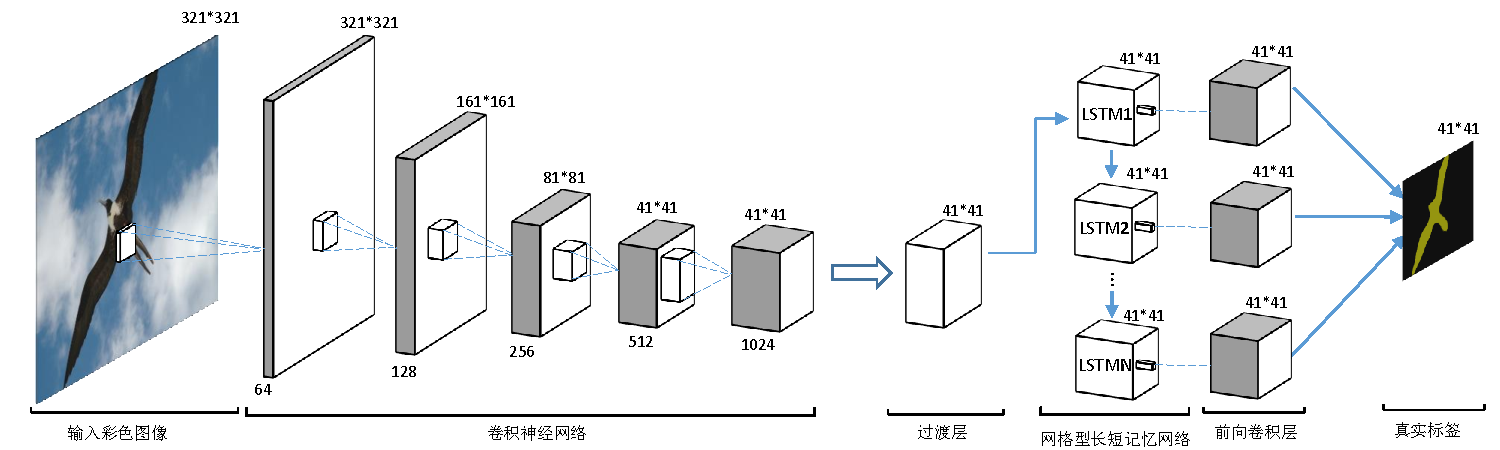
\includegraphics[width=\textwidth]{image/illustration/networkstructure.pdf}
	\end{figure}
}

\frame {
	\frametitle{目录}
	%\begin{multicols}{2}
	\tableofcontents[sections={<1-7>}]
}

%%
% 引言或背景
% 引言是论文正文的开端,应包括毕业论文选题的背景、目的和意义;对国内外研究现状和相关领域中已有的研究成果的简要评述;介绍本项研究工作研究设想、研究方法或实验设计、理论依据或实验基础;涉及范围和预期结果等。要求言简意赅,注意不要与摘要雷同或成为摘要的注解。
% modifier: 黄俊杰(huangjj27, 349373001dc@gmail.com)
% update date: 2017-04-15
%%

\chapter{概述}
%定义,过去的研究和现在的研究,意义,与图像分割的不同,going deeper
\label{cha:introduction}

本章将讲解所做工作的背景、动机, 并与现行已有的解决方案作对比。在分章节中还将对问题作出具体的描述, 并简要介绍本文的工作及论文结构。

\section{背景及动机}
\label{sec:background}
% What is the problem
% why is it interesting and important
% Why is it hards, why do naive approaches fails
% why hasn't it been solved before
% what are the key components of my approach and results, also include any specific limitations,do not repeat the abstract
%contribution
随着新校长的上任, 新校区、新院系的建设如火如荼地进行着, 然而随之而来的是过渡时期旧校区不得不接纳更多待迁移至新校区的新生, 以及宿舍的四人间改六人间、食堂容量的扩增、深圳校区临时教学办公场所建设等的问题。其中很少被人提及, 但却又实实在在地影响着每位学生每天学习、生活体验的就是校园网的网速问题。显然, 在人数增加的情况下, 校园网, 尤其是人数急剧增加的东校区的出口带宽并没有随着之增加, 在网络中心的限速策略下, 校区内人均带宽发生了一定的下降, 在晚上(18:00~24:00)这段网络高峰时间的网络拥堵情况尤为显著, 表现为看网课、游戏主播等直播类应用的卡顿、在线视频应用无法调整为高清分辨率, 自动回落到低分辨率, 游戏因为网络拥塞导致的高延迟等, 都极为影响使用体验\footnote{据SYSU IPv6交流群群友反馈}。

此外, 笔者的同好还向学校网络中心确认了因为出口带宽吃紧导致的校园网IPv6开始正式实施限速措施, 即限速至人均10Mbps\footnote{见附录:《jipeng:关于最近 IPv6 被限速的问题》}\footnote{见附录:《中山大学网络中心: 对事件编号INC000000030481邮件的回复》}, 和之前不限速比起来, 使用体验有着天壤之别。

在此之前, 校内, 尤其是以数据科学与计算机学院院内的一群学生为首的IPv6协议爱好者, 一直致力于在校园内推广IPv6协议应用的使用, 包括但不限于视频直播、文件资源分享、开发镜像CDN等应用类型, 涵盖面广泛, 覆盖了院内学生的诸多需求与现实关切。笔者作为爱好者之一, 深感在学生群体中推广基于IPv6协议应用的必要性, 在养成良好的校内乃至对公网的IPv6协议应用的使用习惯后, 能够使得本来蜂拥至校园网出口的流量变成校园内局域网的流量, 继而大大减轻校园网公网出口的负担, 从而能提供良好的校园网使用体验。

基于上述现实, 笔者及同好们提出了建设一个基于IPv6的资源分享平台的构想, 初步规划使用成熟的Bittorrent协议及相应的客户端软件, 开发一个服务器端的资源分享发布平台, 相比传统的FTP/HTTP等单点C/S、B/S的文件发布分享方式, 具有极好的容错性, 同时Bittorrent协议的分布式特点也能较好地分担各个客户端节点的负担, 使得每位用户都能在较小的性能损耗下收获较好的使用体验。

下面将简要描述国内以IPv6协议推广为目的的大学校内Bittorrent协议资源分享平台现状。

Bittorrent(以下简称BT)作为一种曾经极为流行的文件传输协议, 即使在现在依然有着广泛的用户基础。虽然如今文件分享的主流方式是以百度网盘为首的在线文件存储应用及相关云服务, 但笔者一直相信, 不依赖单一节点的分布式的文件分享才是文件分享的终极方式。国内不少大学的有识之士也认识到这一点, 为此开发、部署、运营着大量的BT资源分享平台。

由于互联网的开放性, 一国国内合法获取的资源在另一国未必具有相应的国内版权, 因此不少BT网站为了规避风险, 将BT分享平台唯一需要中心化部署的追踪器服务器(Tracker)采取账号化管理, 需要注册登录取得相应的鉴权(authentication)方能正常使用 (详细的描述见第二章)。国内大学的BT平台为了规避版权等风险, 不约而同地采取了这样的管理方式。这种管理方式被称作私有追踪器(Private Tracker, 以下简称PT)。PT网站因为需要用户注册登录系统, 以及Torrent文件(种子文件, 以下记作种子)的发布、管理平台, 是需要进行一定的系统分析、调研后去建构及耗时开发的。国内大学的一些团队做了相应的工作, 并将其开源, 被运用在了不少其他大学的PT网站上。

提到国内大学PT网站所用到的系统, 永远无法绕过的是浙江大学Nexus团队开发的NexusPHP\footnote{https://sourceforge.net/projects/nexusphp}系统。以它为基础, 部署、运营、二次开发的代表性PT网站有北京邮电大学的北邮人BYRBT\footnote{https://bt.byr.cn/}, 天津大学的北洋园TJUPT\footnote{https://www.tjupt.org/}等。除了NexusPHP外, 还有以国内最早的教育网\footnote{指早期CERNET骨干网及后期CERNET2这一纯IPv6协议骨干网}PT, 东北大学六维空间\footnote{http://bt.neu6.edu.cn/}为代表的使用开源论坛系统Discuz!\footnote{https://www.discuz.net/}为基础二次开发的PT系统。

目前, 北京邮电大学的北邮人BYRPT和东北大学的六维空间是国内目前最大的教育网内PT网站。

\section{PT网站选型、开发的问题描述}
\label{sec:related_work}
为了能够尽快、可靠地实现前述构想, 笔者及同好必须要在既有的系统中进行选型, 进而二次开发, 尽快上线部署, 赶在新生入学等关键的时间节点进行推广, 进而达到校园网资源最大化利用的目标。开发选型的两个首要选项是1.2中提到的NexusPHP和Discuz!, 两者都是目前比较成熟的PT网站使用的系统, 且都用PHP语言写就。

NexusPHP基于TBSource\footnote{https://sourceforge.net/projects/tbsource/}开发, 在后者的基础上添加或完善了大量功能,同时极大地提高了代码效率(除TBSource外,还吸取了一些其它private tracker的想法或代码,如Bit-HDTV,What.cd和SceneTorrents, 摘自NexusPHP介绍页\cite{nexusteam2011about})。NexusPHP最后一个公开版本发布于2012年7月7日, 版本号为Standard v1.5 Beta 5\footnote{https://sourceforge.net/projects/nexusphp/files/}, 包括北邮人BYRBT在内的国内不少NexusPHP PT网站都是基于这个版本二次开发的。

另一方面, 以六维空间为代表的一类PT网站以成熟的开源论坛系统Discuz!为基础, 利用既有的用户管理功能和附件功能, 在这之上加入流量统计等功能, 使之成为符合PT要求的网站。

然而上述的两个系统都有自己的问题。首先是早期NexusPHP开发的时候, PHP语言的开发范式尚未形成, 许多现代语言的特性, 如包管理、前端解耦、自动构建等系统都没有十分可靠的方案, 成熟的MVC(Model 模型, View 视图, Controller 控制器)框架也未问世, 导致NexusPHP几乎就是在TBSource的基础上继续``裸''写网页。读者不妨想象一下从一无所有的``hello world''程序开始写起到写成DOS系统的过程, 虽然有一定的夸张成分, 但要用早期的PHP标准编写这样网页应用绝非易事, 而在这基础上的二次开发更是难上加难。

事实上, 在同好间早期的网站内部试运营中, 笔者尝试使用了以NexusPHP为基础二次开发的天津大学北洋园TJUPT的开源版本, 其在原始的NexusPHP的基础上美化了样式, 使之更符合现在的审美。然而, 要想在该系统之上进行功能的增删或者调整, 由于代码文件组织结构的不清晰, 以及缺少原始的开发文档等, 诸多变量及方法名都不明晰, 开发难度极大, 因此在之后的选型中被弃用。

而另一个基于Discuz!的PT系统目前鲜有开源版本面世, 介于其本来是为``互联网论坛''这一需求开发的, 不少功能上的冗余需要耗费时间去剔除, 为此期间需要阅读开发文档所带来的时间开销将是相当无用的消耗, 与快速上线的需求不相符。同时, 论坛系统以交流为导向的开发方向与资源分享交流的总目标不甚一致。因此基于上述理由, 笔者未使用Discuz!及其衍生系统进行二次开发。

在既有的开源项目中, 国人作者taobataoma开发的meanTorrent\footnote{https://github.com/taobataoma/meanTorrent}是使用Javascript编写, 以mean(MongoDB\footnote{一种文档式数据库, https://www.mongodb.com/}, Express\footnote{一个使用JavaScript编写的MVC框架, https://expressjs.com/}, Angular.js\footnote{Google公司正在维护的一个渐进式前端框架, https://angularjs.org
/}, Node.js\footnote{一个解释JavaScript语言的后端运行时(Runtime), https://nodejs.org
/})这一相对较多人使用的开发框架组合进行开发。笔者也曾经为其贡献过代码\footnote{https://github.com/taobataoma/meanTorrent/pull/52}, 然而时过境迁, 现在其开发已经陷入沉寂。而且以Node.js开发的网页应用后端系统不可避免地会遇到JavaScript这一纯脚本型语言带来的性能问题。

选型过程中相中的另一个开源项目是目前正在活跃开发的UNIT3D-Community-Edition\footnote{https://github.com/HDInnovations/UNIT3D-Community-Edition}, 由美国开发者HDVinnie发起。该项目使用PHP编写, 以成熟的Laravel框架为基础开发, 前端框架可以使用时下正红的React\footnote{https://reactjs.org/}或者Vue\footnote{https://vuejs.org/
}, 具有良好的用户界面(User Interface, 以下简称UI), 并且前后端解耦, 代码组织结构清晰, 变量方法名命名规范, 能够自我解释, 进行二次开发的难度最小, 同时Demo网站\footnote{https://unit3d.site/}已经具有不错的用户体验, 因此笔者最终选择使用UNIT3D-Community-Edition(以下简称UNIT3D)进行二次开发。

\section{本文的工作}

通过将既有的UNIT3D Demo网站投入试运营, 收集内测人员的意见反馈, 针对性地根据校园网使用场景进行功能增删调整等的二次开发。增删调整的功能中, 包括但不限于:

\begin{enumerate}[label=\arabic*.,leftmargin=*]
\item 完善UI的中文语言本地化(Localization)工作
\item 数据库表字段的调整
\item 从前述NexusPHP内测系统的数据迁移
\item 标签系统的调整优化
\item 投票桩功能的系统实现
\item 反作弊用的IP地址记录功能
\end{enumerate}


\section{论文结构简介}

\label{sec:arrangement}
本文第一章首先简要介绍了中山大学校园网, 尤其是东校区校园网出口带宽紧张的现状, 进而提出构建运营一个校园内部分布式资源分享平台的构想, 列举比较了当前被国内大学广泛使用的基于分布式BT协议的PT网站及其所用的系统软件, 即NexusPHP与Discuz!, 并对比了另外两种开源项目meanTorrent及UNIT3D, 经过权衡取舍, 最终将二次开发的原型选型定为UNIT3D。

第二章将主要介绍为了进行二次开发而需要的相关技术, 包括Bittorrent协议, Trac\-ker服务器软件要求, Private Tracker的要求, BT客户端软件, 使用PHP编写的Laravel MVC框架, 以及将要基于其二次开发的使用Laravel框架编写的UNIT3D项目。

第三章将介绍针对试运营过程中发现的问题以及收集到的反馈意见, 所将要进行的二次开发的开发任务。首先要将前期试运营使用的NexusPHP的数据库表迁移至UNIT3D的数据库中, 为此需要对UNIT3D的数据库字段进行相应的调整。在使用的过程中, 发现其投票系统是仅打桩未实现的功能, 进而进行具体而完整的实现, 使之能与NexusPHP的投票功能相媲美。最后根据PT的反作弊需要实现了部分IP地址记录的功能。此外还有小规模的标签系统调整。

第四章将描述针对第三章中总结出的开发任务所进行的具体实现, 包括关键代码的一些展示及解释。

第五章将对论文的成果进行展示。

第六章将分析讨论本论文成果的优缺点, 并对中山大学校园PT网站的前景进行展望。


\section{深度神经网络}
\frame
{
  \frametitle{\secname~ }
  \begin{block}{前馈神经网络}
	  传统的人工神经网络
  \end{block}
  \begin{block}{卷积神经网络}
	  目前最为流行的,广泛应用于视觉任务的神经网络
  \end{block}
  \begin{block}{长短记忆网络}
	  与卷积网络相比,更适用于处理时序信号
  \end{block}
}
\subsection*{深度神经网络}
\frame{
	\frametitle{前馈神经网络结构}
    \begin{columns}[onlytextwidth]
		\begin{column}{0.5\textwidth}
			\vspace{-1.5em}
		\begin{itemize}
			\item 有向无环图的结构
			\item 输入层(数据特征)
			\item 隐含层(映射后的特征)
			\item 输出层(预测结果)
			\item 反向传播算法(训练方法)
		\end{itemize}
		\end{column}
		\begin{column}{0.5\textwidth}
		\begin{figure}[h] %structure of LSTM
			\centering
			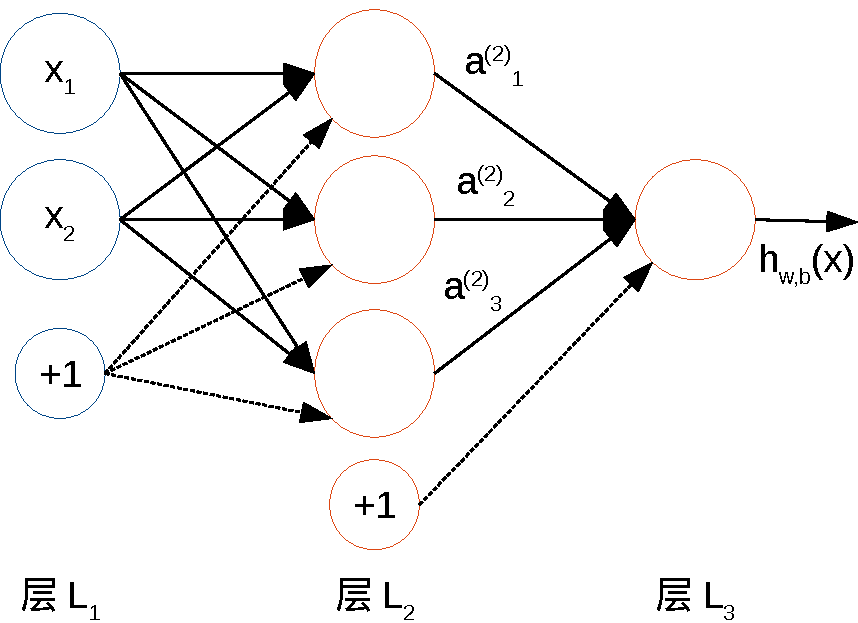
\includegraphics[width=0.9\textwidth]{image/illustration/network1.pdf}
			\caption{前馈神经网络模型示意图}
			\label{fig:lstm}
		\end{figure}
		\end{column} 
	\end{columns}
}

\frame{
   \frametitle{卷积神经网络}
   \vspace{-0.8em}
	\begin{figure}
		\centering
		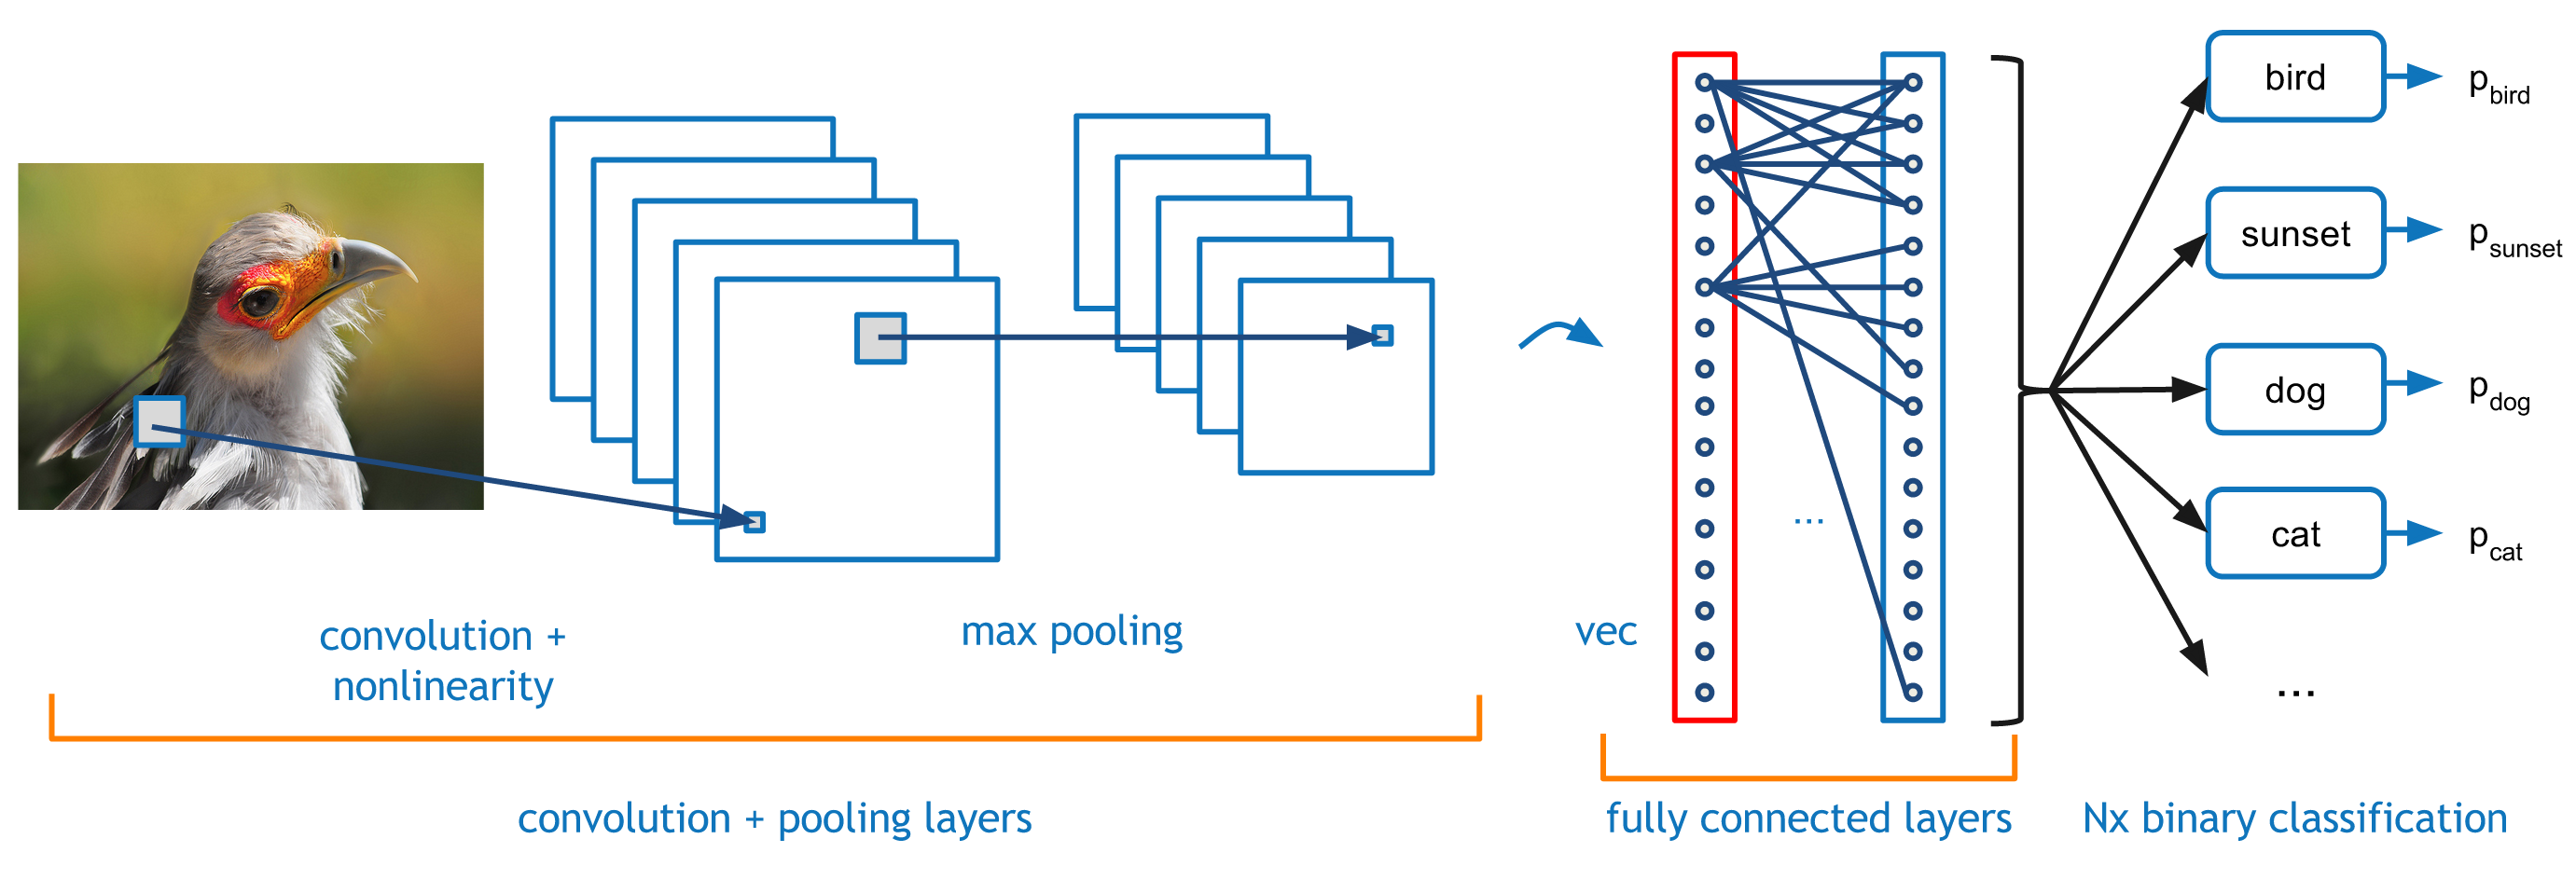
\includegraphics[width=0.8\textwidth]{figures/CNN}
		\caption{卷积网络模型示意图}
		\label{fig:network1}
	\end{figure}  
   \vspace{-0.8em}
	\begin{block}{与前馈神经网络的区别}
	\begin{itemize}
		\item 直接作用于二维图像,无需特征设计阶段
		\item 卷积层,池化层
		\item 局部感知域,权重共享
	\end{itemize}
	\end{block}
}

\frame{
	\frametitle{长短记忆网络(处理一维信号)}
	\tiny
	\vspace{-2em}
    \begin{columns}[onlytextwidth]
        \begin{column}{0.5\textwidth}
	    \begin{figure}[h] %structure of LSTM
	    	\centering
	    	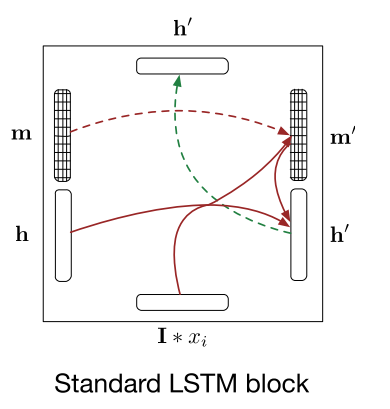
\includegraphics[width=0.6\textwidth]{figures/lstmblock1}
	    	\caption{长短记忆网络区块示意图}
	    	\label{fig:lstm}
	    \end{figure}
		\end{column} 
		%%%%%%% new column
		\begin{column}{0.5\textwidth}
			\begin{boxedminipage}{0.8\textwidth}
			\vspace{-1.5em}
			\begin{align}
				\label{eq:lstm}
				\begin{split}
				\textbf{g}^u &= \delta(\textbf{W}^u*\textbf{H}) \\
				\textbf{g}^f &= \delta(\textbf{W}^f*\textbf{H}) \\
				\textbf{g}^o &= \delta(\textbf{W}^o*\textbf{H}) \\
				\textbf{g}^c &= \mbox{tanh}(\textbf{W}^c*\textbf{H}) \\
				\textbf{m}' &= \textbf{g}^f \odot \textbf{m} + \textbf{g}^u \odot \textbf{g}^c \\
				\textbf{h}' &= \mbox{tanh}(\bf{g}^o \odot \bf{m}') \\
					\textbf{H} & = \begin{bmatrix}
					I*\textbf{x}_i \\ \textbf{h}
					\end{bmatrix}
			\end{split}
			\end{align}
		\end{boxedminipage}
		\end{column}
    \end{columns}
	
	\vspace{-1em}
	\begin{block}{缩写形式}
	\footnotesize
	\begin{equation*}
		(\textbf{h}', \textbf{m}') = \mbox{LSTM}\bigr(\textbf{H},\textbf{m},\textbf{W} \bigr)
	\end{equation*}
	其中\textbf{W}包含了四个门权值矩阵$\textbf{W}^u,\textbf{W}^f,\textbf{W}^o,\textbf{W}^c$。
	\end{block}
}

\frame{
	\frametitle{网格型长短记忆网络(处理N维信号)}
	\vspace{-1.5em}
	\begin{figure}[h]
	\centering
		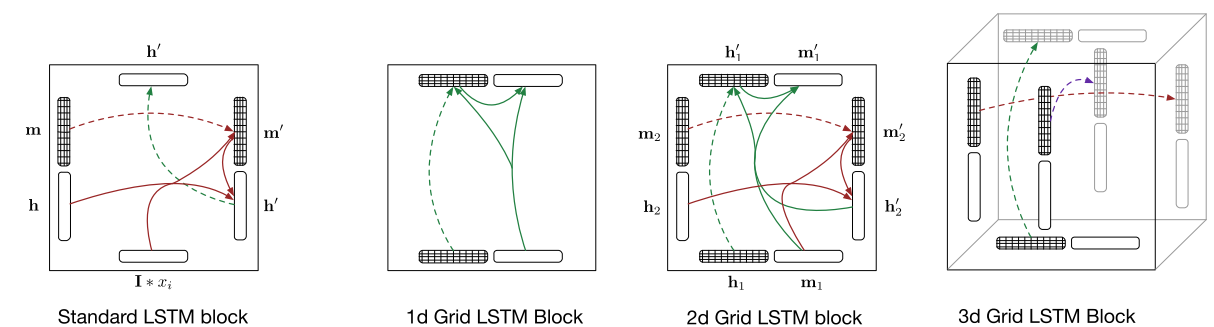
\includegraphics[width=\textwidth]{figures/gridlstm}
		\caption{网格型长短记忆网络区块示意图[Kalchbrenner et al, Grid LSTM, ICLR 2016]}
	\end{figure}
	\vspace{-2em}
	\begin{block}{网格型长短记忆网络更新过程}
	\tiny
	\begin{columns}[onlytextwidth]
		\begin{column}{0.4\textwidth}
		\vspace{-0.5em}
			\begin{equation}
				\textbf{H} = \begin{bmatrix}
					\textbf{h}_i \\ \vdots \\ \textbf{h}_N
				\end{bmatrix}
			\end{equation}
		\end{column}
		\begin{column}{0.6\textwidth}
		\vspace{-1em}
			\begin{align}
				\begin{split}
				(\textbf{h}_1', \textbf{m}_1') & =  \mbox{LSTM}(\textbf{H}, \textbf{m}_1, \textbf{W}_1) \\ &\mbox{ }\vdots \\
				(\textbf{h}_N', \textbf{m}_N') & =  \mbox{LSTM}(\textbf{H}, \textbf{m}_N, \textbf{W}_N)
				\end{split}
				\label{eq:gridlstm}
			\end{align}
		\end{column}
	\end{columns}
	\end{block}
}
\endinput

\section{网络模型结构}
\subsection*{网络模型结构}
\frame{
  \frametitle{网络整体结构}
	\begin{figure}[h]
		\centering
		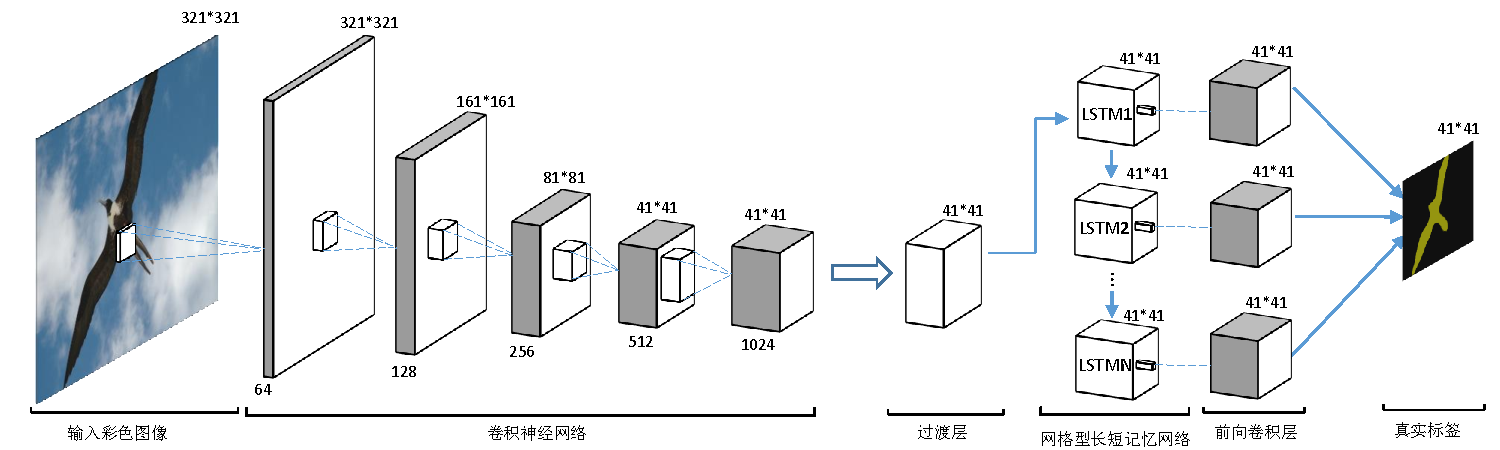
\includegraphics[width=0.9\textwidth,height=0.28\textwidth]{image/illustration/networkstructure.pdf}
		\caption{网络整体结构图}
		\label{fig:networkstructure}
	\end{figure}
	\vspace{-1em}
	\small
	\begin{block}{}
	\begin{itemize}
		\item  四个组成部分:\textbf{卷积网络部分},过渡层,\textbf{网格型长短记忆网络部分},前向卷积层
		\item 核心思想:在卷积网络后堆叠多层网格型长短记忆层
	\end{itemize}
	\end{block}
}
\frame{
	\frametitle{卷积网络部分}
	\vspace{-1em}
	\footnotesize
	\begin{block}{}
	\begin{itemize}
		\item 基于$VGG_{16}$模型\footnote{Simonyan \& Zissermanet, Very deep Convolutional Networks For Large-scale Image Recognition, ICLR 2015}, 含有16层卷积层
		\item 使用了“孔算法”,在不损失精度的情况下将模型参数减少了 6.5 倍\footnote{Chen et al, DeepLab-LargeFOV, ICLR 2015}
	\end{itemize}
	\end{block}
	\vspace{-1em}
	\begin{figure}[h]
		\centering
		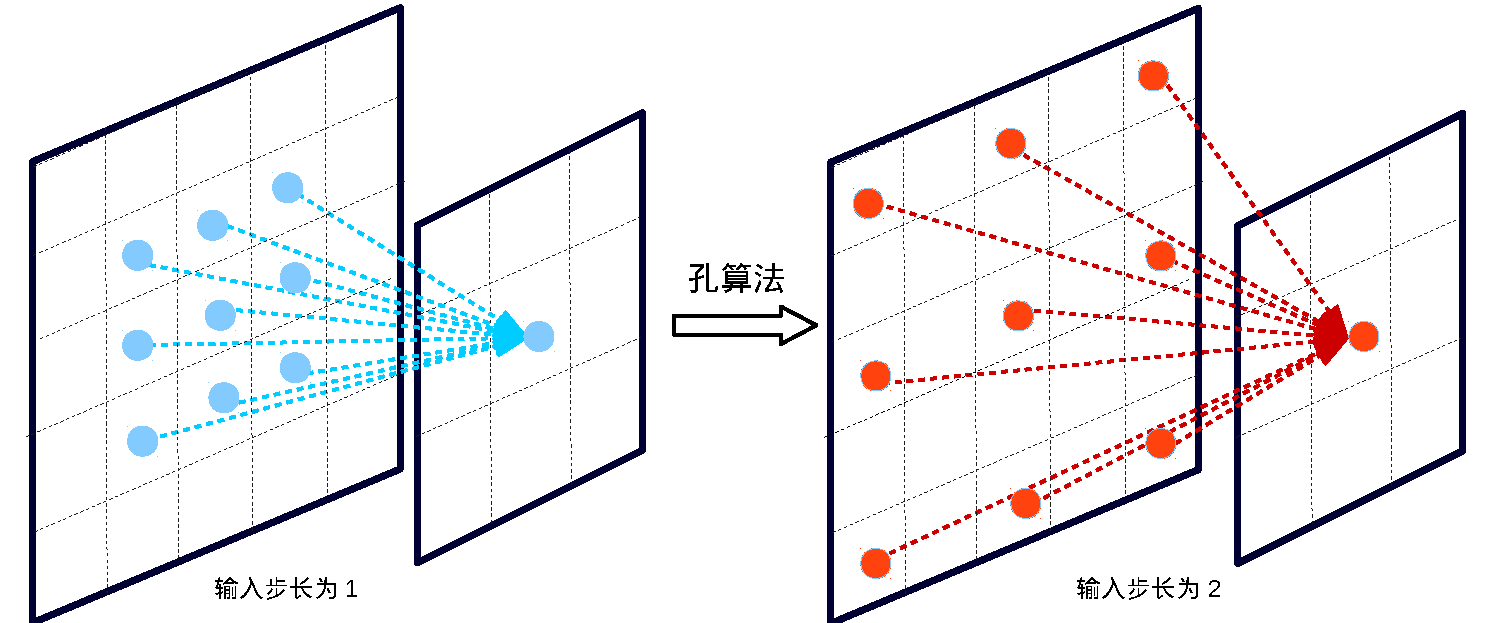
\includegraphics[width=0.7\textwidth]{image/illustration/hole.pdf}
		\caption{"孔算法"示意图}
	\end{figure}
}

\frame{
\frametitle{网格型长短记忆网络部分}
	\vspace{-1em}
    \begin{columns}%[onlytextwidth]
        \begin{column}{0.6\textwidth}
        \vspace{0.2em}
		\begin{figure}
			\centering
			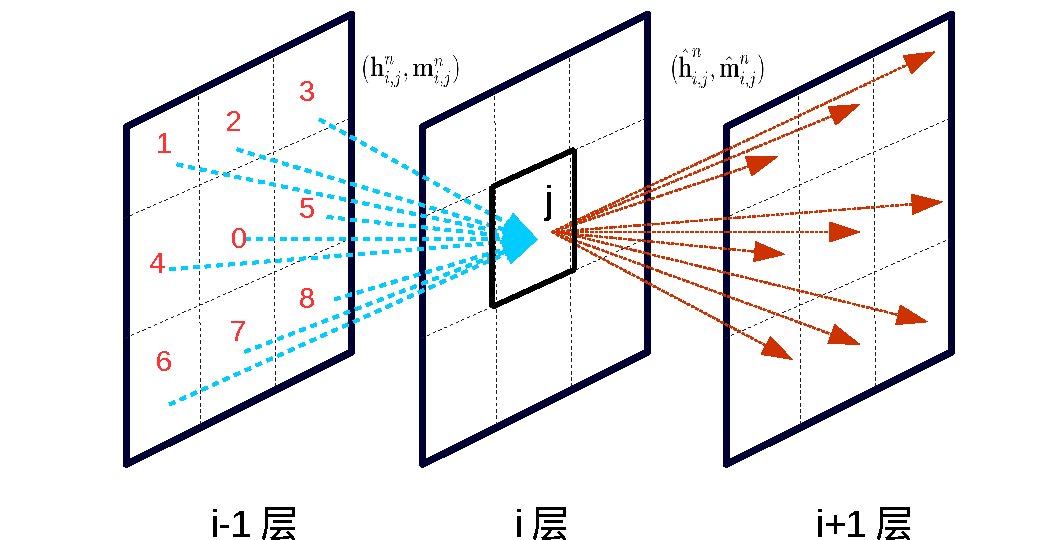
\includegraphics[width=\textwidth]{image/illustration/neighboring.pdf}
			\caption{九维网格型长短记忆网络层之间的通信示意图}
			\label{fig:neighboring}
		\end{figure}
		\end{column} 
		%%%%%%% new column
		\begin{column}{0.5\textwidth}
			\footnotesize
			\vspace{-1.5em}
			\begin{align}
				\begin{split}
				(\hat{\textbf{h}}_{i,j}^0,\hat{\textbf{m}}_{i,j}^0) &= \mbox{LSTM}(\textbf{H}_{i,j},\textbf{m}_{i,j}^0,\textbf{W}_i) \\
				(\hat{\textbf{h}}_{i,j}^1,\hat{\textbf{m}}_{i,j}^1) &= \mbox{LSTM}(\textbf{H}_{i,j},\textbf{m}_{i,j}^1,\textbf{W}_i) \\
				\vdots \\
				(\hat{\textbf{h}}_{i,j}^N,\hat{\textbf{m}}_{i,j}^N) &= \mbox{LSTM}(\textbf{H}_{i,j},\textbf{m}_{i,j}^N,\textbf{W}_i) \\
				\textbf{H}_{i,j} &= [\textbf{h}_{i,j}^0\mbox{ }\textbf{h}_{i,j}^1\mbox{ }...\mbox{ }\textbf{h}_{i,j}^N]^T
				\end{split}
			\end{align}
		\end{column}
    \end{columns}
	\footnotesize
	\vspace{-1em}
	\begin{block}{九维网格型长短记忆网络}
		\vspace{-0.7em}
		\begin{itemize}
			\item 每个位置的预测会受到上一层相邻八邻域特征的影响
			\item 随着层数的堆叠,每一位置将会有更大的感知域。
			\item 网格型长短记忆网络的层数通过实验来确定
		\end{itemize}
	\end{block}
}



%% chapter 4 dataset, network structure, experiment and result
\chapter{PT网站的具体实现、改进与运营}
\label{cha:experiment}

在本章中, 将着重详细介绍前一章中提出的开发计划如何具体落地实施。同时, 在运营方面, 将介绍一些内测人员招募、培养用户习惯的实践经验。能够将自己的兴趣爱好推荐给他人, 并能使他人受益, 这样的课外实践令笔者收获了颇多心得。

\section{部署开发、运行、测试环境}

开发环境使用的是捷克Jetbrain公司的PhpStorm IDE(Integrated Development Environment, 集成开发环境)。它拥有完善的词头联想及代码补全功能, 能够极大地提高开发效率。

\begin{figure}[ht]
    \centering
    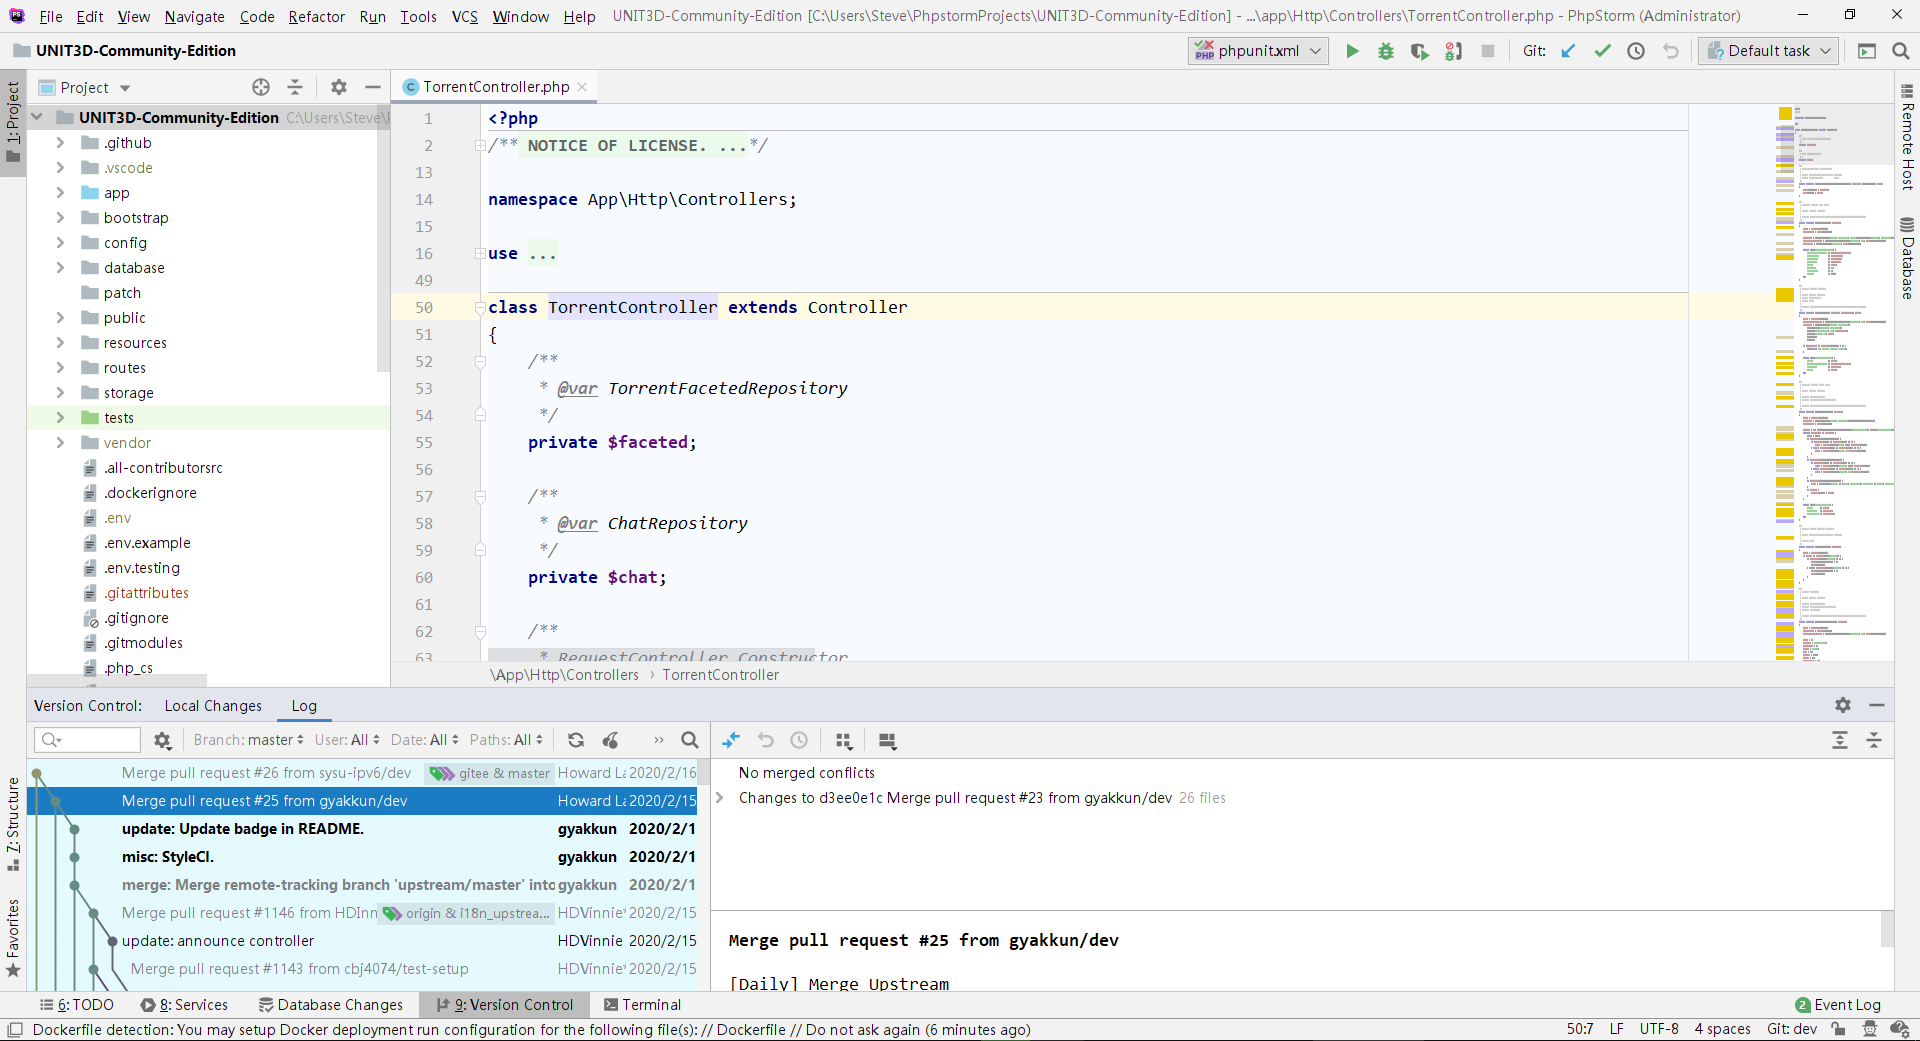
\includegraphics[width=0.8\textwidth]{support-files/4.1-phpstorm-ide.png}
    \caption{PhpStorm IDE}
    \label{fig:phpstormide}
\end{figure}

UNIT3D作者提供了一份手动部署的手册, 以及一个自动部署脚本, 但与当前各依赖包的最新版本有所脱节。为此, 笔者使用了站长howardlau同学提供的Dockerfile, 在每一次代码的修改、提交、推送之后, 交由代码托管方github的自动工作流系统\footnote{\url{https://help.github.com/en/github/collaborating-with-issues-and-pull-requests/github-flow}进行Docker\footnote{https://www.docker.com/}}镜像的构建与发布。若构建失败笔者将会收到邮件通知, 从而分载(Offload)了部分本应人工完成的编译时(Compile-time)测试工作。

\begin{figure}[ht]
    \centering
    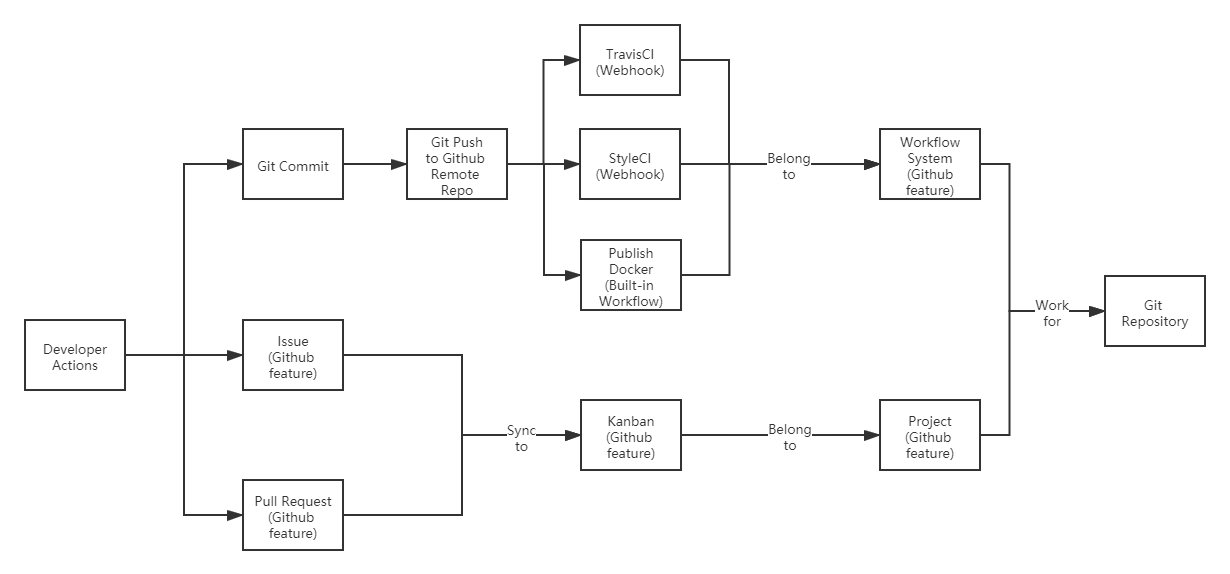
\includegraphics[width=\textwidth]{support-files/4.1-github-workflow.png}
    \caption{Github 工作流系统示意图}
    \label{fig:githubworkflow}
\end{figure}

% [图 (4.1-github-workflow) GITHUB 工作流 流程图]

除此之外, 笔者还使用了TravisCI\footnote{\url{https://travis-ci.org/}}进行部分用例测试, StyleCI\footnote{\url{https://styleci.io/}}来检查代码格式规范。两者都是各自领域优秀的持续集成(Continuos Integration, CI)测试工具, 基本上承担了大部分代码级别的测试工作, 效果见图 \ref{fig:ci}。具体的功能测试将在\ref{sec:preop}中的试运营部分给出描述。

\begin{figure}[h]
	\centering
    \begin{subfigure}{0.8\textwidth}
		\centering
		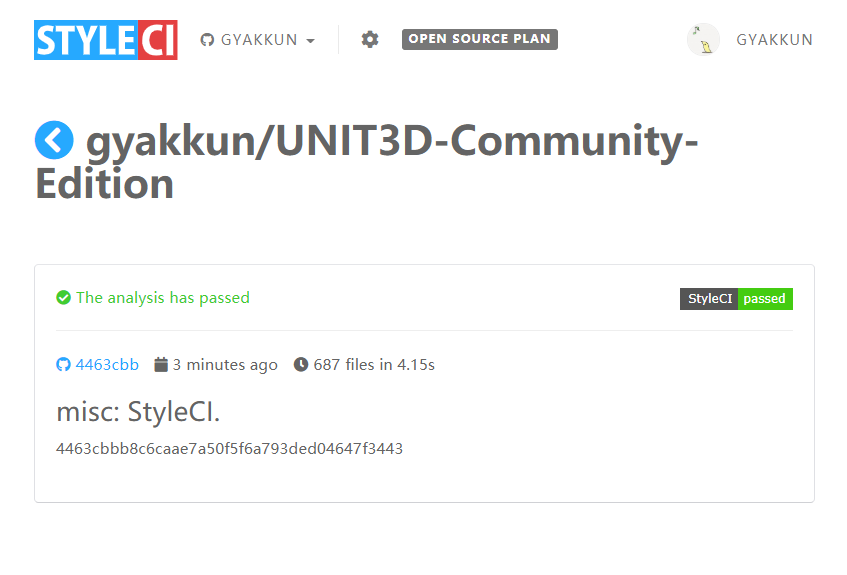
\includegraphics[width=\textwidth]{support-files/4.1-style-ci.png}
		\caption{StyleCI}
		\label{fig:styleci}
    \end{subfigure} \\
    \vbox{}
    % 全角空格占位, 否则空不出两行
     \\
    \vbox{}
	% \makebox[0.05\textwidth]{}
    \begin{subfigure}{0.8\textwidth}
		\centering
		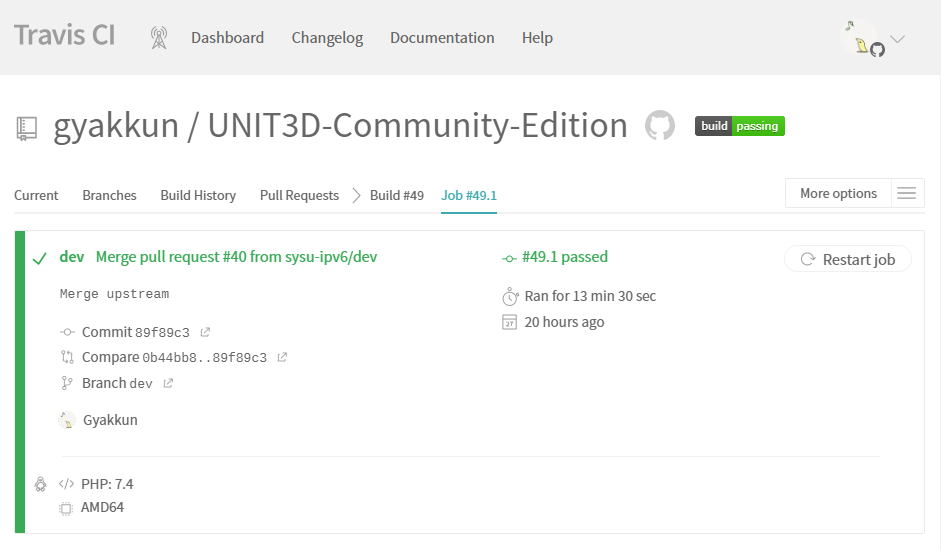
\includegraphics[width=\textwidth]{support-files/4.1-travis-ci.png}
		\caption{TravisCI}
		\label{fig:travisci}
	\end{subfigure} 
    % \makebox[0.05\textwidth]{}
    \caption{两种在线持续集成工具}
	\label{fig:ci}
\end{figure}

% [图 (4.1-style-ci, 4.1-travis-ci) TravisCI StyleCI]

具体的本地测试环境是在VMware虚拟机上, 通过PhpStorm的Deploy(部署)功能以及虚拟机的SSH(Secure shell, 安全外壳协议)服务, 能够将代码实时地从本地开发环境同步到虚拟机的测试环境中。然后在本地开发环境的浏览器中就能实时预览到开发中的网页, 见图 \ref{fig:devenv}。

\begin{figure}[h]
	\centering
    \begin{subfigure}{0.8\textwidth}
		\centering
		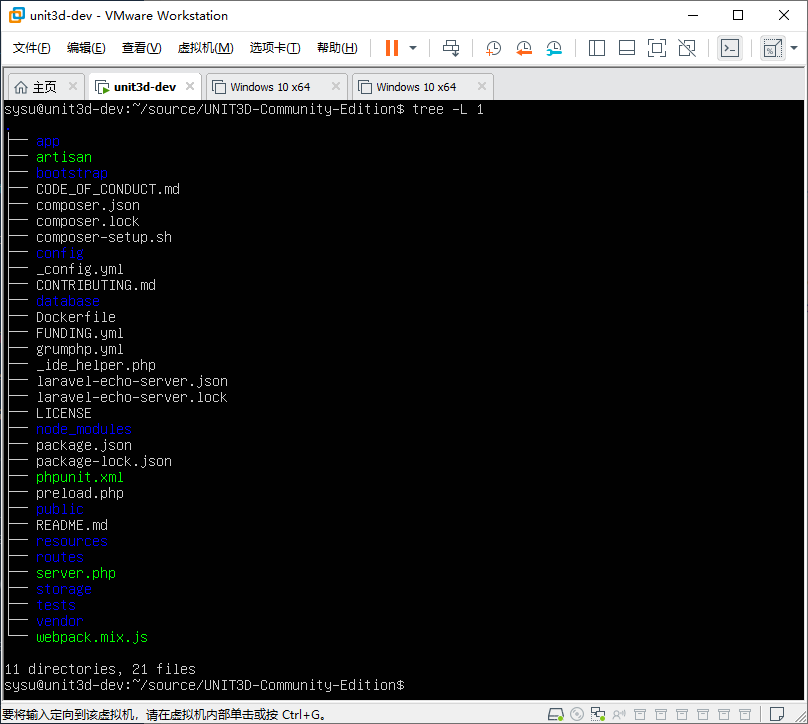
\includegraphics[width=\textwidth]{support-files/4.1-vwmare-unit3d-dev.png}
		\caption{VMware 下看到的目录结构}
		\label{fig:vmware}
	\end{subfigure} \\
	% \makebox[0.05\textwidth]{}
    \begin{subfigure}{0.8\textwidth}
		\centering
		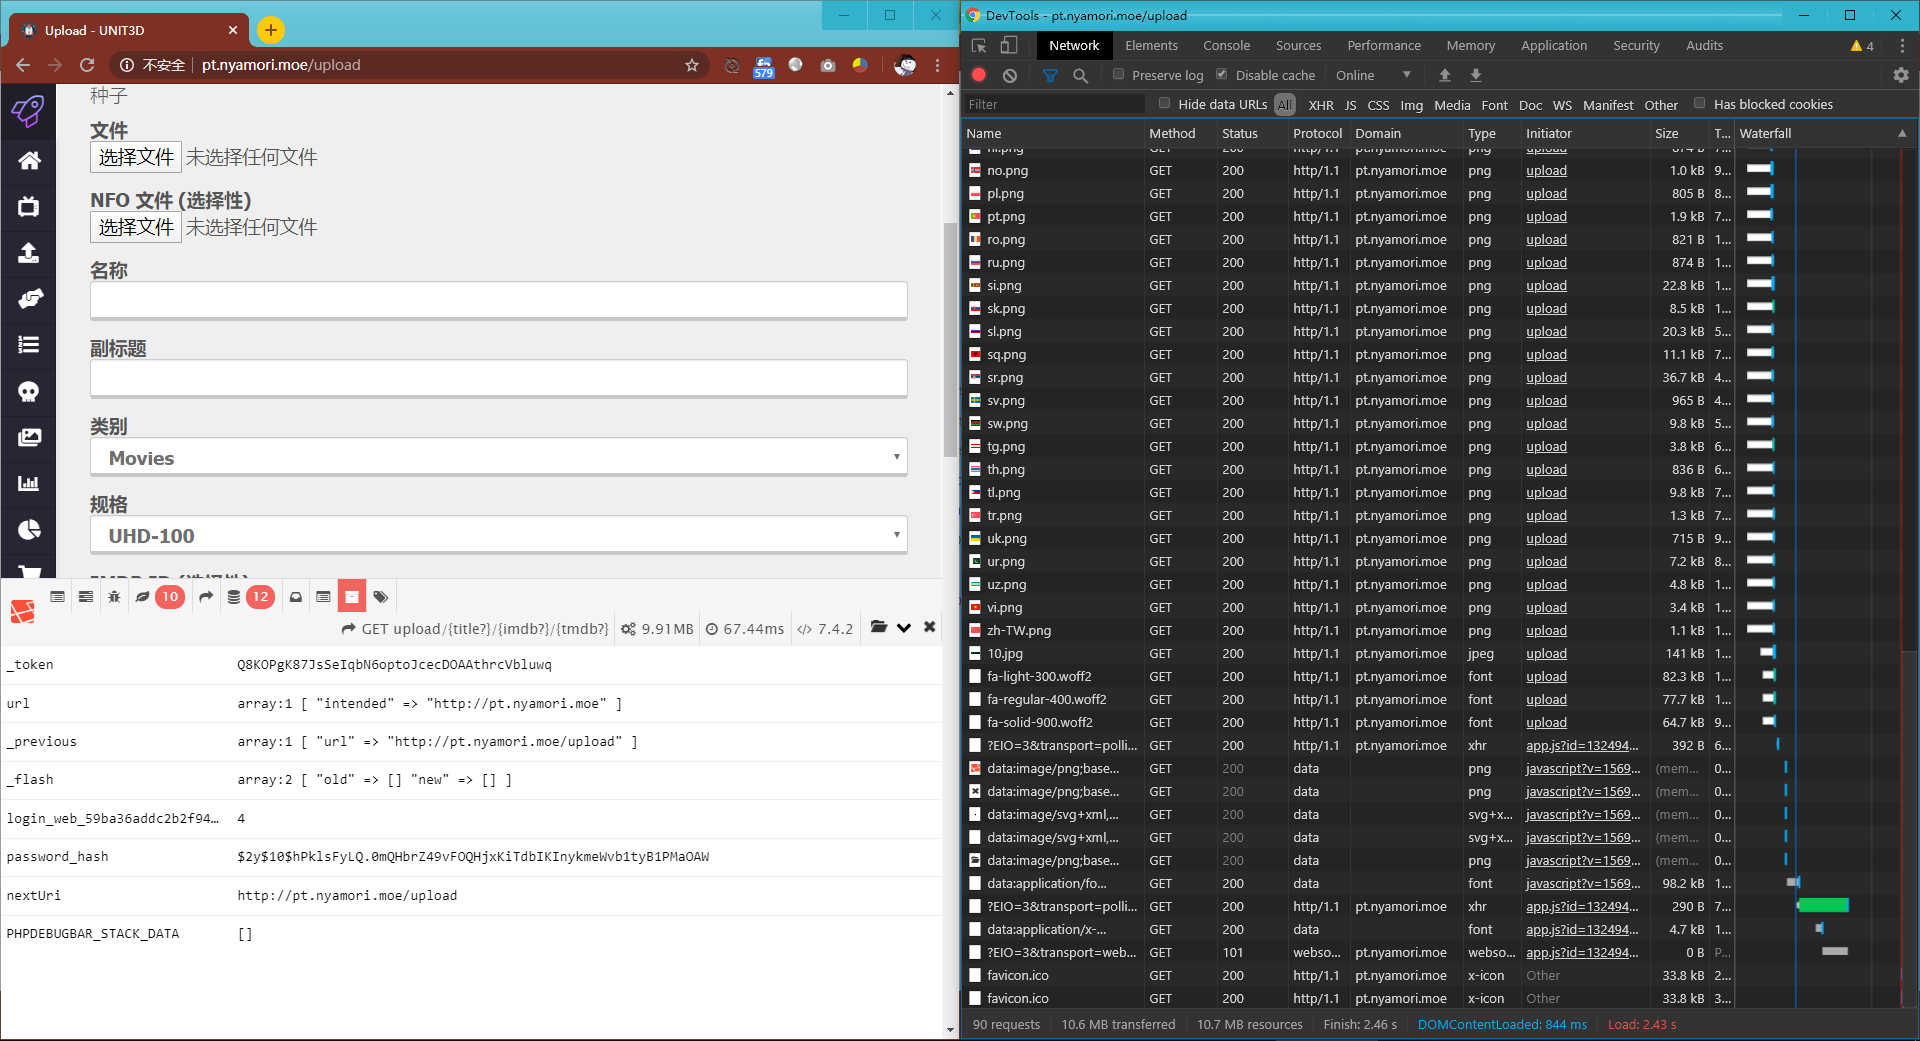
\includegraphics[width=\textwidth]{support-files/4.1-web-idehelper-chrome-devtool.png}
		\caption{调试中的网页}
		\label{fig:chromedevtool}
	\end{subfigure} 
    % \makebox[0.05\textwidth]{}
    \caption{调试环境}
	\label{fig:devenv}
\end{figure}

% [图 (4.1-vwmare-unit3d-dev, 4.1-web-idehelper-chrome-devtool) 虚拟机 和 调试阶段的页面 截图重点给到IDE HELPER 和网页下面的Dev Toolbar]

\section{本地化工作}

Laravel框架具有较好的国际化兼容性, 通过在资源文件中定义相应英文单词的特定语言翻译, 然后在视图模板文件中使用`@lang('app.langItem')'这种注记将原始内容表示出来, 就可以简单地通过前端的语言切换选项切换所渲染的不同语言界面。

\begin{figure}[ht]
    \centering
    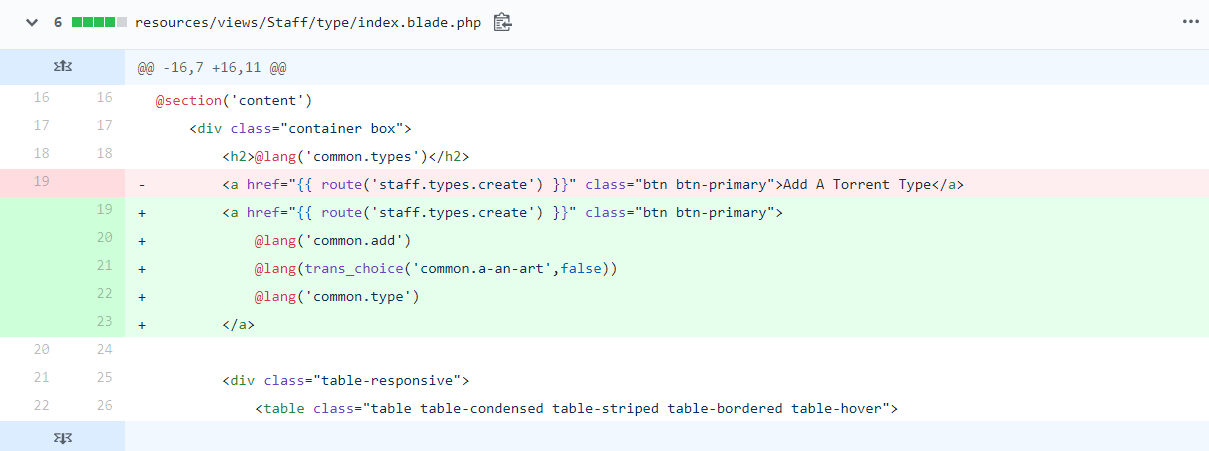
\includegraphics[width=0.9\textwidth]{support-files/4.2-git-diff.png}
    \caption{本地化所做的代码修改}
    \label{fig:localdiff}
\end{figure}

% [图 (4.2-git-diff) 一份git diff式的源码前后对比, 突出从原始英语单词到`@lang('app.langItem')'的部分]

针对英语转中文的翻译部分, 由于笔者曾经修过实用口译这门课程, 对快速高效的翻译颇有心得。经过一番重新翻译、修改、润色, 最终得到了令人满意的中文用户界面。

\begin{figure}[h]
	\centering
    \begin{subfigure}{0.3\textwidth}
        \centering
        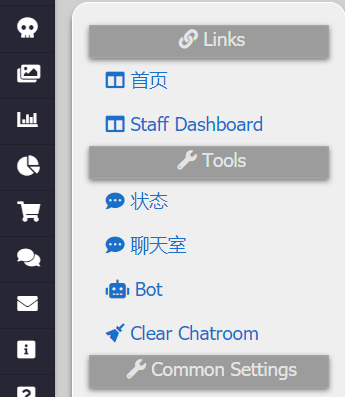
\includegraphics[width=\textwidth]{support-files/4.2-before-localization-cut.png}
        \caption{本地化前}
        \label{fig:beforelocal}
    \end{subfigure}
    \makebox[0.05\textwidth]{}
    \begin{subfigure}{0.3\textwidth}
        \centering
        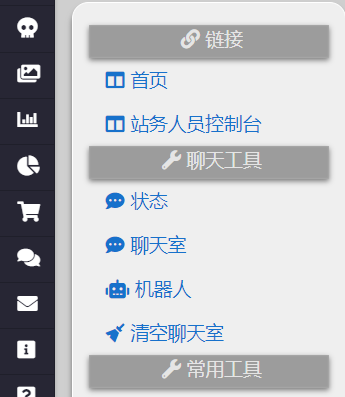
\includegraphics[width=\textwidth]{support-files/4.2-after-localization-cut.png}
        \caption{本地化后}
        \label{fig:afterlocal}
    \end{subfigure} \\
    % \makebox[0.05\textwidth]{}
    \caption{本地化前后的站务工作台页面对比}
    \label{fig:guidifflocal}
\end{figure}

% [图 (4.2-before-localization-cut, 4.2-after-localization-cut) 对比前后用户界面的语言部分]


\section{数据表迁移工作}
\label{sec:migration}

迁移脚本实际上就是将原表的字段一一对应到新表的字段中, 然后通过SQL语句逐条地重新录入。

前置步骤是将新表建立起来。这里用到了Laravel自带的`Illuminate\textbackslash Database\textbackslash Sche\-ma\textbackslash'类提供Migration子类。实际上, 所有数据库迁移操作基本都离不开对这个类类方法的使用。下图所示是给UNIT3D表结构中新增副标题(Subhead)字段的迁移脚本。

\begin{figure}[ht]
    \centering
    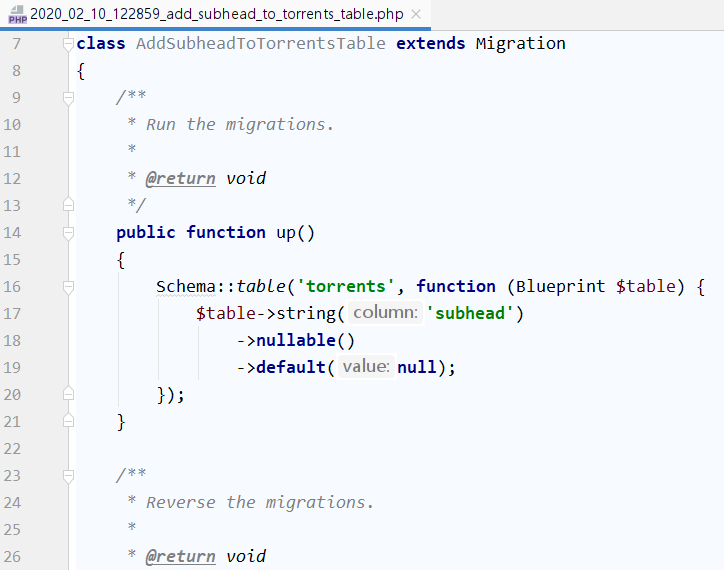
\includegraphics[width=0.9\textwidth]{support-files/4.3-subhead-migration-script.png}
    \caption{增加Subhead字段所用的迁移脚本}
    \label{fig:subheadmigratescript}
\end{figure}

% [图 (4.3-subhead-migration-script) 新表中新增subhead的脚本, 截图/database/migrations/2020\_02\_10\_122859\_add\_subhead\_to\_torrents\_table.php]

在这里, Blueprint类会将相应的Migration类方法, 比如`\$table->string('subhead')', 转化为SQL语句`alter table \$table add subhead', 从而达到增加字段的目的。

同时, Migration子类中定义了回溯的`down()'函数, 方便进行数据库迁移失败后的反向迁移。

具体的从NexusPHP迁移到UNIT3D的脚本, 包含了一个创建新表的脚本, 用到上述Blueprint类的子类方法, 按照目标的表结构创建数据表。还包含了一个描述新旧数据表各字段映射关系的`Mapping.php'文件, 里面的代码负责将旧表中的每一行数据解析, 转换成新表对应字段的`INSERT'SQL语句, 然后执行, 从而达到旧表迁移到新表的目的。

\begin{figure}[ht]
    \centering
    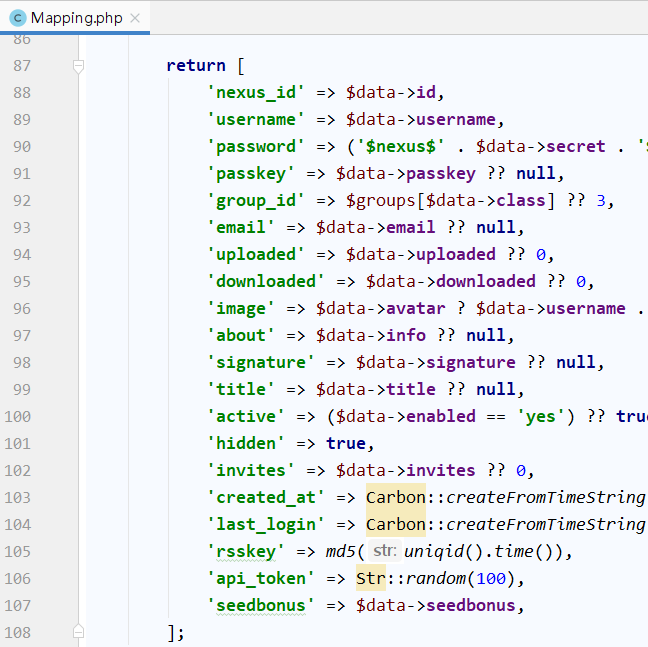
\includegraphics[width=0.6\textwidth]{support-files/4.3-tjupt-to-unit3d-script-mapping.png}
    \caption{新旧数据表的映射关系}
    \label{fig:mapnexusphpunit3d}
\end{figure}

% [图 (4.3-tjupt-to-unit3d-script-mapping) 旧表 vs 新表, 截取PHPSTORM中TJUPT\_TO\_UNIT3D中的Mapping.php]


\section{功能删改 - 标签功能调整}

事实上, \ref{subsec:tagadjust}中所描述的标签系统问题, 很大程度是因为UNIT3D数据表维护的种子元信息中, 有不少字段被设置为"必填项"。比如电影种子的`IMDB ID'项就属于对笔者一方非必要的字段, 但因为被设置为必填项, 故在测试阶段只能填无实际语义的样例值, 或者直接填0主动触发报错。该值又与标签系统向IMDB API的请求参数直接相关, 导致部署测试运行过程中的大量报错。

找到问题的原因之后, 笔者先尝试剔除诸如上述"电影"资源分类中`IMDB ID'字段的必要输入开关。其后, 因为在\ref{sec:migration}所描述的数据表迁移中, 为新表增加了很多其他资源类型项, 因此, 只要将自带的电影等分类从数据库中删除, 将新的分类设置成默认分类, 即可绕过上述标签的联网获取机制, 变相达到剔除标签功能的目的。

\begin{figure}[ht]
    \centering
    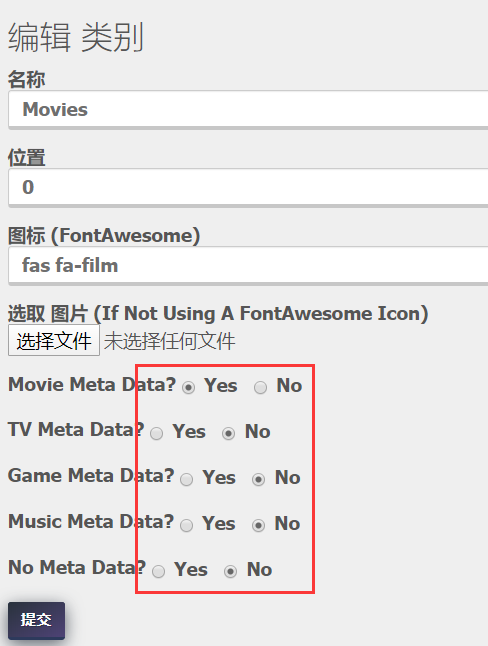
\includegraphics[width=0.45\textwidth]{support-files/4.4-remove-requirement-for-tag-system.png}
    \caption{取消必要字段开关}
    \label{fig:disableforcemeta}
\end{figure}

\section{功能增添 - 投票功能的实现}

投票功能可以用在统计信息, 收集用户意见, 交由用户对网站内外的大事小情进行表态, 从而决定网站的运营、开发方向, 是实用性相当高的一个功能。该功能未能具体完整地实现, 不得不说是UNIT3D原版的一大缺憾。

UNIT3D的数据库中定义有poll和voters两个数据表。乍一看很容易混淆, 实际上poll里的项代表被发起的一次投票, voters的项则代表每人次投出去的票, 记录着投票人、投票选项以及投票时发起的HTTP请求的源IP地址。同时, 为了记录投票的选项, 还使用一张option表来存储每个投票的选项。

UNIT3D原版实现了增加单项投票的功能。然而, 删/改投票, 多选投票, 以及投票的重复IP检查功能都尚处于桩函数的状态, 相关的网页前端只留了一个`\#'的空锚点, 并无有效超链接路径。为此, 笔者对投票的删除、修改, 多选投票, 以及投票的重复IP检查进行了具体的实现。

\subsection{投票的删除、修改}

投票的增删改主要涉及到`/app/Http/Controllers/Staff/PollControler.php'这个控制器以及`/resources/views/Staff/poll/'下的相应视图模板。

对于控制器, 笔者增加了`update(\$id)', `destroy(\$id)'函数。其中`update(\$id)'函数包含了对既有投票的修改。`destroy(\$id)'则根据投票的唯一ID在数据库中删除相应的投票。

在修改投票的过程中, 管理员可能增加/删除/修改既有的选项名称。为此, 需要从前端请求中获取相应的选项ID, 然后比对数据表中相应ID的既有选项名称是否和前端返回的选项名称一致, 若不一致, 则将其加入临时待增加/修改/删除选项数组中, 在之后的循环中逐一从数据库中增加/修改/删除。流程图见图 \ref{fig:updateflowchart}。

这里用到了不少前端的技巧。为了使前端的修改请求能够带上原始选项的ID, 笔者在控制器返回给前端的修改投票页面里的具体各个投票的区块中, 增加了非显示字段`poll-id'以及`option-id', 顾名思义, 就是数据表中对应投票/选项的唯一ID。在前端将要提交的表单中, 这两项会一并提交, 从而在后端的控制器中能取到相应的ID, 继而进入上述`update(\$id)'函数的流程中。

\begin{figure}[h]
    \centering
    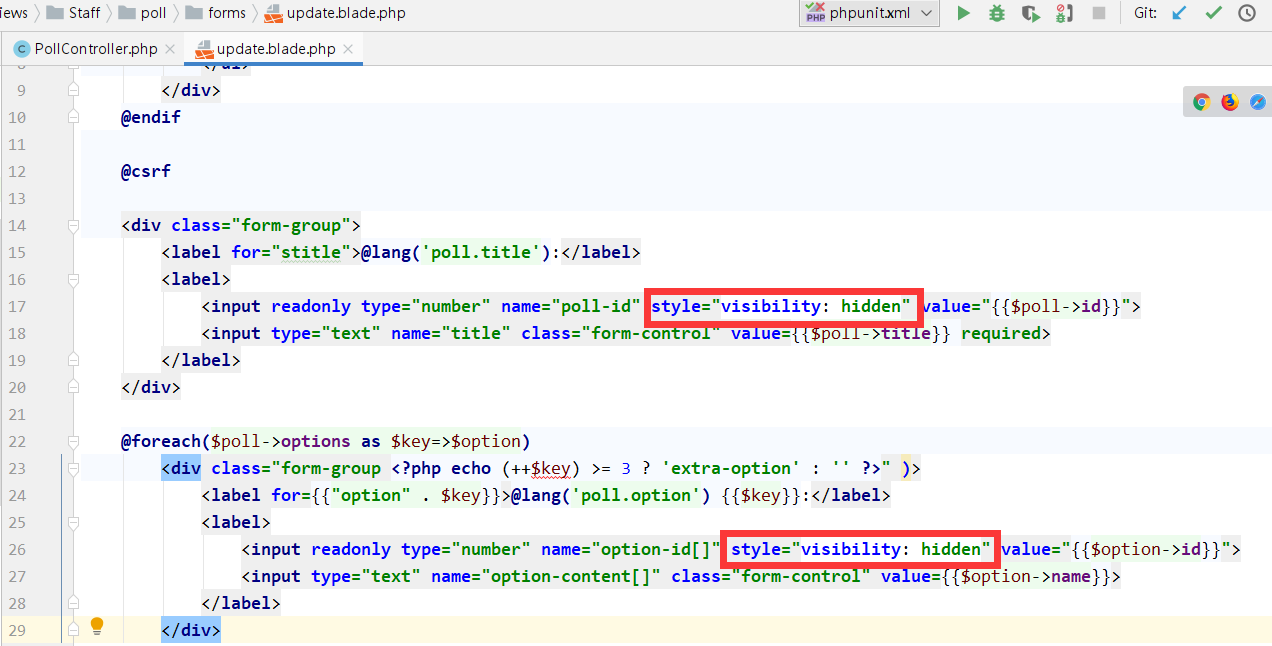
\includegraphics[width=0.8\textwidth]{support-files/4.5.1-visibility-hidden.png}
    \caption{在模板中设置visibility:hidden}
    \label{fig:visibilityhidden}
\end{figure}

删除的逻辑类似, 从前端取得待删除的投票ID后, 交由Laravel的模型模块, 自动注入相关类方法, 继而从数据表中实际删除对应的投票。

\begin{figure}[hbp]
    \centering
    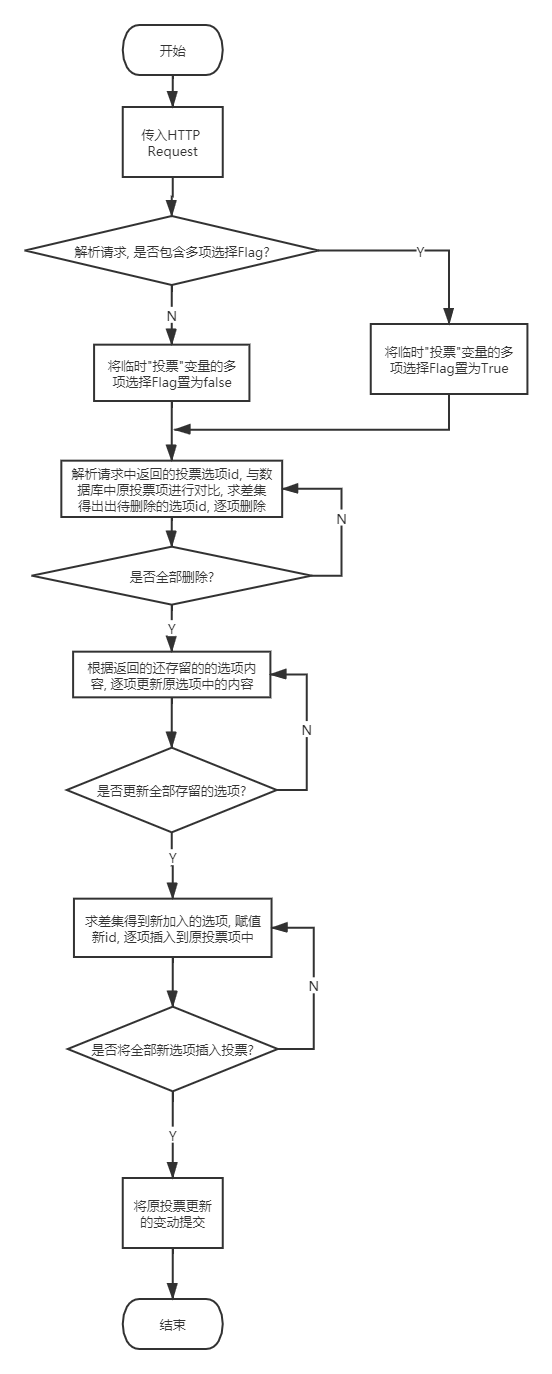
\includegraphics[width=0.37\textwidth]{support-files/4.5.1-pollcontroller-update-flowchart.png}
    \caption{update()函数的流程图}
    \label{fig:updateflowchart}
\end{figure}

\newpage

\subsection{投票的重复IP校验}

重复IP校验的逻辑并不复杂, 只要将每次投票的HTTP请求中的源IP提取出来, 再与voter数据表中相应poll\_id外键对应的所有票的ip字段进行比对, 若发现一致的, 则判定为重复IP。

\begin{figure}[hb]
    \centering
    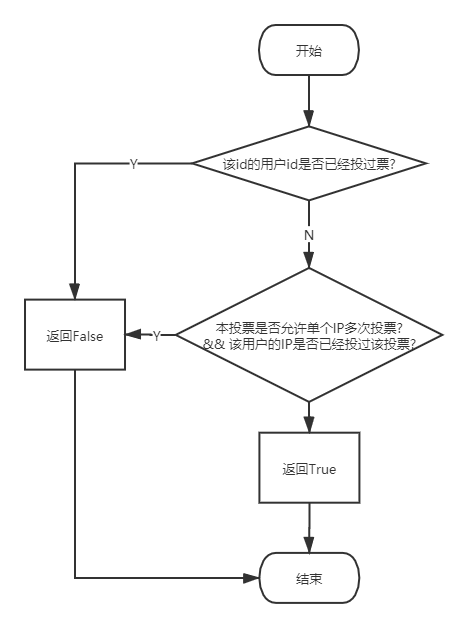
\includegraphics[width=0.2\textwidth]{support-files/4.5.2-validate-voter-flowchart.png}
    \caption{validateVoter()函数的流程图}
    \label{fig:validatevoterchart}
\end{figure}

% [图 (4.5.2-validate-voter-flowchart) 判定重复IP流程图 app\textbackslash Http\textbackslash Controllers\textbackslash PollController.php  validateVoter()函数]

具体的实现中, 使用了或非运算符简化运算, 但语义不太明晰。

\begin{figure}[h]
    \centering
    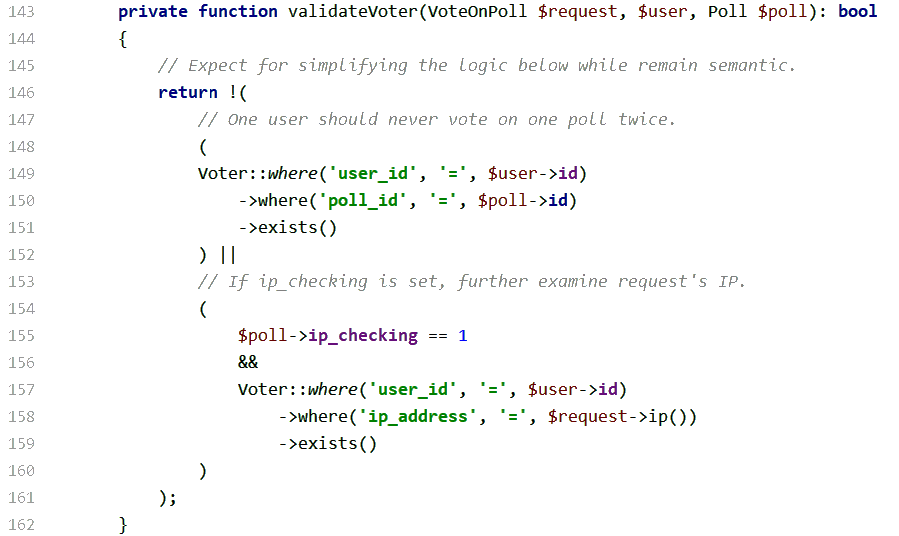
\includegraphics[width=0.8\textwidth]{support-files/4.5.2-validate-voter-code.png}
    \caption{validateVoter()函数的具体代码}
    \label{fig:validatevotercode}
\end{figure}

% [图  (4.5.2-validate-voter-code) 直接糊代码 app\textbackslash Http\textbackslash Controllers\textbackslash PollController.php  validateVoter()函数]


\section{功能增添 - 初步添加鉴权操作日志记录功能}

由于\ref{subsec:auth}中描述的理由, 需要为系统添加鉴权操作日志功能(以下记作``鉴权日志")。鉴权日志需要定义一个全新的数据模型, 并对应一张新的数据表, 因此需要进行一定的上层设计及数据库的迁移。

\subsection{数据模型的定义}

因为主要记录的是鉴权操作, 而HTTP服务器软件, 比如nginx\footnote{\url{https://www.nginx.com/}}, 都有独自完善的日志功能, 所以本平台的鉴权日志只需记录用户相关的信息, 以及根据用户所用的设备等具有辨识性质信息哈希得到的一个识别码。为此, 定义Authentication类, 记录'user\_id', 'device\_id','ip\_address'三个字段, 分别对应PHP的integer, integer和string原生类型。为了记录鉴权的状态, 定义三种字符串常量, 'LOGIN', 'FAILED', 'LOCKOUT', 分别表示登录(即鉴权成功), 失败(表示当此鉴权操作失败, 如密码错误), 以及锁定(账户多次鉴权操作失败, 账户被上锁, 待解封) 之后的持久化步骤交给Laravel的持久化模块。

\begin{figure}[h]
    \centering
    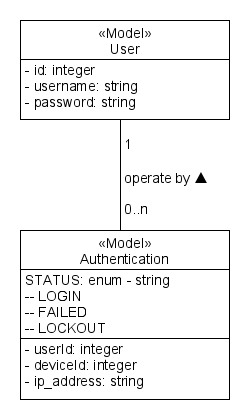
\includegraphics[width=0.45\textwidth]{support-files/4.6.1-authentication-model-png.png}
    \caption{User类和Authentication类的E-R图}
    \label{fig:userauthmodeler}
\end{figure}

% [图 (4.6.1-authentication-model-png) models/authentication.php 可以用UML画E-R图]


\subsection{数据库迁移脚本}

为了记录前述的数据模型, 要在数据库中定义新的数据表。这里用到前述的数据库迁移脚本。只需要将新字段的名称和SQL数据类型通过Blueprint类的相应子类类方法告知数据库即可。

\begin{figure}[h]
    \centering
    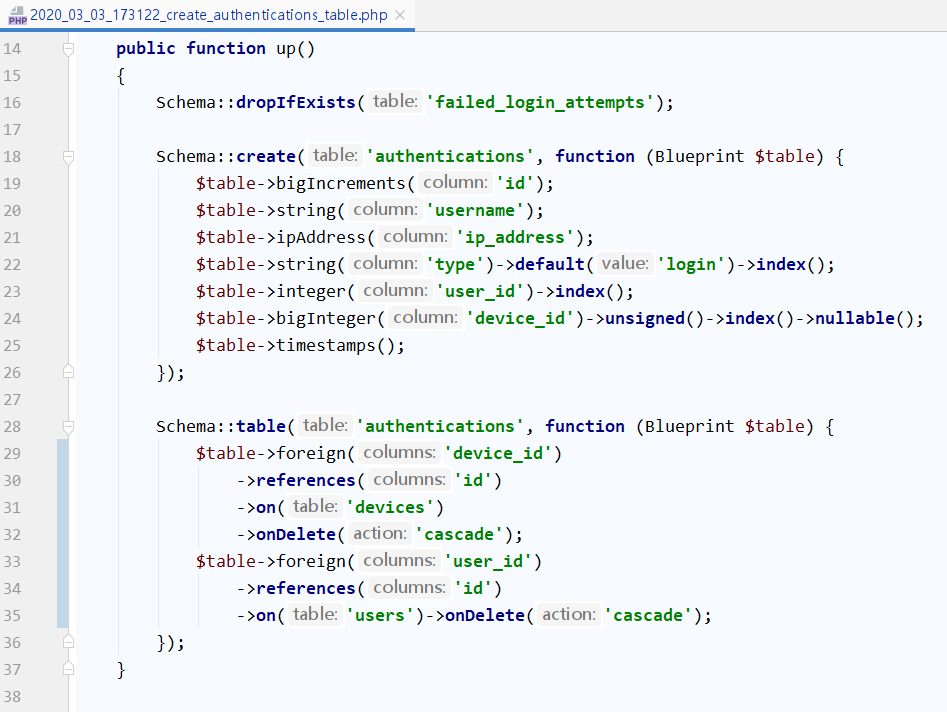
\includegraphics[width=0.8\textwidth]{support-files/4.6.1-migration-script.png}
    \caption{针对Authentication表的数据库迁移脚本}
    \label{fig:authmigratescript}
\end{figure}

% [图 (4.6.1-migration-script) \textbackslash database\textbackslash migrations\textbackslash 2020\_03\_03\_173122\_create\_authentications\_table.php]

\subsection{具体的日志记录逻辑}

为了实现日志记录, 需要为每一次鉴权操作注册监听事件。为此需要在Laravel框架中的事件监听服务中注册鉴权操作的事件订阅者(AuthEventSubscriber), 流程图如下。

% [图 (4.6.3-event-model) 摘要Laravel的事件监听机制]


\section{网站的上线部署}

网站的上线主要是站长17级软件工程专业的howardlau同学在负责。具体的上线方式是采用Docker部署, MySQL数据库和Redis缓存服务也使用既有的Docker镜像, 通过"docker-compose"\footnote{\url{https://docs.docker.com/compose}}将其组合成容器, 方便今后交付到诸如Kubernete等的容器化云平台上投入生产使用。

\section{试运行}
\label{sec:preop}

笔者及同好通过SYSU IPv6交流群\footnote{一个群员以中山大学数据科学与计算机学院学生为主的兴趣交流QQ群}以及相关公众号推送\footnote{微信公众号: SYSPT}招募内测用户。用户群体主要是数据科学与计算机学院的学生, 他们对BT协议以及PT网站都有一定的了解, 有些还是北邮人BYRBT和六维空间的忠实用户。对于这样内测用户, 不用重新培养使用习惯, 能够较好地帮助运营方确定用户需求, 并得以迅速跟进开发实现。

而对另一部分通过推送慕名而来的BT新手, 笔者及同好还有数据科学与计算机学院的热心同学们热情地为他们提供了帮助。通过这样良好的内部交流, 循环促进培养新人的用户习惯, 整个网站的建设正在有条不紊地推进中。

\chapter{网站效果展示}

本章将主要展示已经部署上线的网站UI, 以及相应的资源发布、下载、查找的简明步骤, 以期读者能够通过对本章的阅读迅速掌握网站的使用方法。

\section{网站的用户界面}

用户首页, 有聊天盒、推荐种子等功能。左侧的一栏图标代表资源搜索下载、上传等细分功能。

[图 (5.1-index-ui) 首页]

\section{资源的查找与下载}

点击左侧的"资源"图标, 进入搜索页。在搜索框内输入关键字, 无需点按搜索按钮, 马上自动响应发起搜索请求。

[图 (5.2-search-page-1) 简单搜索页]

如对搜索结果不满意, 或是要进行进一步的筛选, 可使用右上角的筛选器按钮, 进行高级搜素。

[图 (5.2-search-page-2) 高级搜索页]

在搜索结果列表点击想要下载的资源, 进入种子详情页面。

[图 (5.2-torrent-detail-page) 种子详情页]

\section{资源的发布}

点击页面左侧的资源发布图标, 进入资源发布页面。输入相应的种子描述信息后即可发布。

[图 (5.2-upload-page) 资源发布页]

\section{BT客户端的使用}

种子文件下载到本地后, 使用BT客户端打开。如图所示为qBittorrent\footnote{\url{https://www.qbittorrent.org/}}。

[图 (5.4-bt-client-1) 选择需要下载的文件]



%%
% 结论
% 结论是毕业论文的总结,是整篇论文的归宿,应精炼、准确、完整。结论应着重阐述自己的创造性成果及其在本研究领域中的意义、作用,还可进一步提出需要讨论的问题和建议。
% modifyer: 黄俊杰(huangjj27, 349373001dc@gmail.com)
% update date: 2017-04-13
%%

\chapter{总结与展望}


\section{本文工作的总结}

随着百度网盘的一家独大, 国内的在线文件分享服务格局从微博微盘, 华为Vdisk, 115网盘, 360云盘等多家服务提供商百花齐放, 竞争到如今基本只有百度和115能在较高收费的基础上提供高质量的在线文件存储、分享服务的格局。加之近日(2020年4月16日)有新闻报道百度网盘的限速策略破解软件PanDownload的作者被警方逮捕[注], 中文互联网的文件分享格局面临进一步的失控, 一旦百度公司宣布旗下的网盘服务停止运营或是大规模收费, 那对全中国互联网网民来说将是一个重大的利空。因此, 去中心化的文件存储、分享服务在笔者看来很有必要, 且势在必行。而BT作为成熟可靠的协议, 在过去的十数年间已有极为成功的网民间自发推广使用的历史。本文的工作目标便是将这一协议的价值重新发掘出来, 配以一个在线资源发布分享平台, 推广该协议在校内的使用。

在初期的开发选型过程中, 笔者及同好所在的团队经历过反复, 先选用了NexusPHP的衍生品天津大学北洋园TJUPT进行二次开发, 察觉到其巨大的二次开发难度后, 遂经过比较后转用UNIT3D, 随后开发步入正轨。

在数据的迁移过程中, 笔者通过使用修改适配后的数据库迁移脚本, 将原来NexusPHP上的数据表迁移至UNIT3D的数据表中, 并增加了必要的字段, 使用户能够较为无痛地从旧系统迁移至新系统。

在随后的功能完善实现中, 笔者剔除了不必要的标签系统功能, 完善实现了投票功能, 初步实现了鉴权操作日志记录功能。这些功能的调整为之后的上线内测运营打下了基础。

在一群行动力极强的同好的共同帮助下, 网站得以迅速上线运行。从初版基于天津大学北洋园TJUPT程序二次开发而来的网站于2019年12月19日上线, 到1月[????]日网站转向使用UNIT3D-Community-Edition作为服务程序, 到今天(2020年4月18日), 共发展了[???? 超过500?]位用户, 有着[???? 600]个资源。随着新学期的开始, 相信在强有力的校内推广下, 会逐渐发展出成熟、稳定的用户群。

笔者作为开发者参与了整个网站建设的全过程, 从初期站长突如其来地上线[注: 2019年12月19日, 21weeks.icu正式上线内测], 到站务、开发团队的招募与组建, 随后的开会讨论网站的技术转型, 再到NexusPHP转UNIT3D等的一系列工作, 无不饱含着每一位同好倾注的心血。

\section{本文工作的优缺点}

本文提出及实现实现到最终上线运营的资源分享平台, 具有如下优点:

\begin{enumerate}[label=\arabic*.,leftmargin=*]
\item UI美观。较其他大学流行的基于NexusPHP的PT网站有更加清晰的逻辑入口, 还包括响应式的自适应UI, 为手机用户浏览本站提供了一定的兼容性。

\item 稳定可靠。基于PHP语言的Laravel框架受益于其以来的PHP-FPM[注]运行时的所有优良特性, 包括进程式的请求响应管理, 将系统出错造成的损失局限在单独的进程之内, 相比如Node.js等因使用单线程处理事件循环[注]而需要更高成本的故障转移(Failover)的计算资源管理方式, 更不容易因为单点故障而导致网站可用性的下降(Degrade)。

\item 易于开发。Laravel框架的设计模式, 包括服务提供者(ServiceProvider), 事件机制, 以及完善自解释的MVC模型, 都为开发者提供了友好的开发体验。这为能够快速实现需求提供了难易度上的保证。

\item 已进入实际运营。与部分只停留在纸面上的论文不同, 作为工程类的论文, 本文的工作成果已经投入了实际的运营中[注 https://21weeks.icu/]。随着用户群的稳步扩张, 加上即将开学[注: 本文写于2020年4月19日]带来的新的一轮推广及用户招募, 本文的工作将会在更广阔的范围内显示其价值。

\item 持续完善中。本文所描述的资源分享平台在将来也会进行更多功能上的改进, 而非止步于本文列举的工作。在毕业后, 相信除了笔者以外, 会有更多志同道合的伙伴会加入到本项目的开发、运营、维护中来, 本文的工作也因此能得以持续完善。
\end{enumerate}


与此同时, 本文的工作也存在着不足, 包括:
\begin{enumerate}[label=\arabic*.,leftmargin=*]
\item NexusPHP的部分功能, 如页面小游戏功能和竞猜功能, 没能在这轮开发中得以迁移。因此新旧两版网站的用户体验并非无缝过渡。

\item 本文所做的工作之一的鉴权日志, 目前尚未实现前端的查询, 需要使用SQL终端或是SQL的管理用工具(如 MySQL Workbench[注]), 以及配合HTTP服务器本身的日志记录功能, 方可实现对鉴权日志的筛查。
\end{enumerate}

包括以上优缺点在内的特点既是本文笔者自豪的地方, 也是遗憾所在。

\section{展望}

文件分享, 作为计算机应用典型中的典型, 自互联网诞生以来, 就是所有网络用户需求之中最基础、也是最关键的一类。从最早的FTP协议, 到通过HTTP协议提供文件服务, 再到去中心化的BitTorrent, 以及今天衍生出的更彻底的去中心化协议IPFS[注], 不依赖Tracker、基于DHT[注]的BitTorrent协议, 还有结合了HTTP和BT优点的基于WebRTC的Web Seed技术一直在进步, 不论是网民自发推动的, 还是商业公司发起并推广甚至开源的。毫无疑问, 文件分享作为互联网的基础应用, 将长久地留存在所有互联网用户的使用习惯当中。

BitTorrent协议, 以及其标准中定义的Tracker服务器, 曾在很长一段时间内都是互联网文件分享的事实标准之一。至今仍有大量的BT用户活跃在世界各地, 秉持着分享精神这一人类的美好品质, 为有需要的人提供他们想要的资源。

本文所做的, 不过是站在BT协议这一巨人的肩膀之上, 在一所大学校园内, 建设了一个为校内用户使用的资源分享平台。与前人栽树的努力相比, 可以说是坐地乘凉般不足为道的微小工作。

然而笔者相信, 本文的工作必将有它巨大的价值。笔者坚信, 只要BT协议的使用习惯一旦形成, 将难以割舍, 用户群的分享精神将会得到激发。网盘固然好, 但资源的命脉始终被扼在一家以商业利益为终极目标的公司手中, 并不可靠。BT作为互联网分享精神的代表, 终将展现出其无限的潜能。

希冀于BT再一次在神州大地上开花结果!



% \chapter{总结与展望}
% \section{工作总结}
% \section{研究展望}
% \section{模板提供的命令}
% 冒号前面是命令,后面是显示的结果\\

% pozhehao(破折号):\pozhehao \sysuspace mybold\{com\}(加粗斜体):\mybold{com} \sysuspace  etoday:\etoday\sysuspace ctoday:\ctoday\sysuspace


% 用于equation环境的命令

% $norm :\norm{t}$

% $argmax:\argmax{x}{y}\sysuspace argmin:\argmin{x}{y}$

% $varmax:\varmax{x}{y}\sysuspace  varmin:\varmin{x}{y}$

% $fncmax:\fncmax{x}{y}\sysuspace  fncmin:\fncmin{x}{y}$

% $xxFnorm:\xxFnorm{x}\sysuspace xxFnormSqr:\xxFnormSqr{x}\sysuspace xxFprod:\xxFprod{x}{y}$

% $xxOpVec:\xxOpVec{x}\sysuspace xxLprod:\xxLprod{x}{y}\sysuspace xxLprodVec:\xxLprodVec{x}{y}\sysuspace xxTensor:\xxTensor{x}$

% $xxBracketY:\xxBracketY{x}\sysuspace xxBracketF:\xxBracketF{x}\sysuspace xxBracketH:\xxBracketH{x}$

% \begin{figure}
% 	\centering
% 	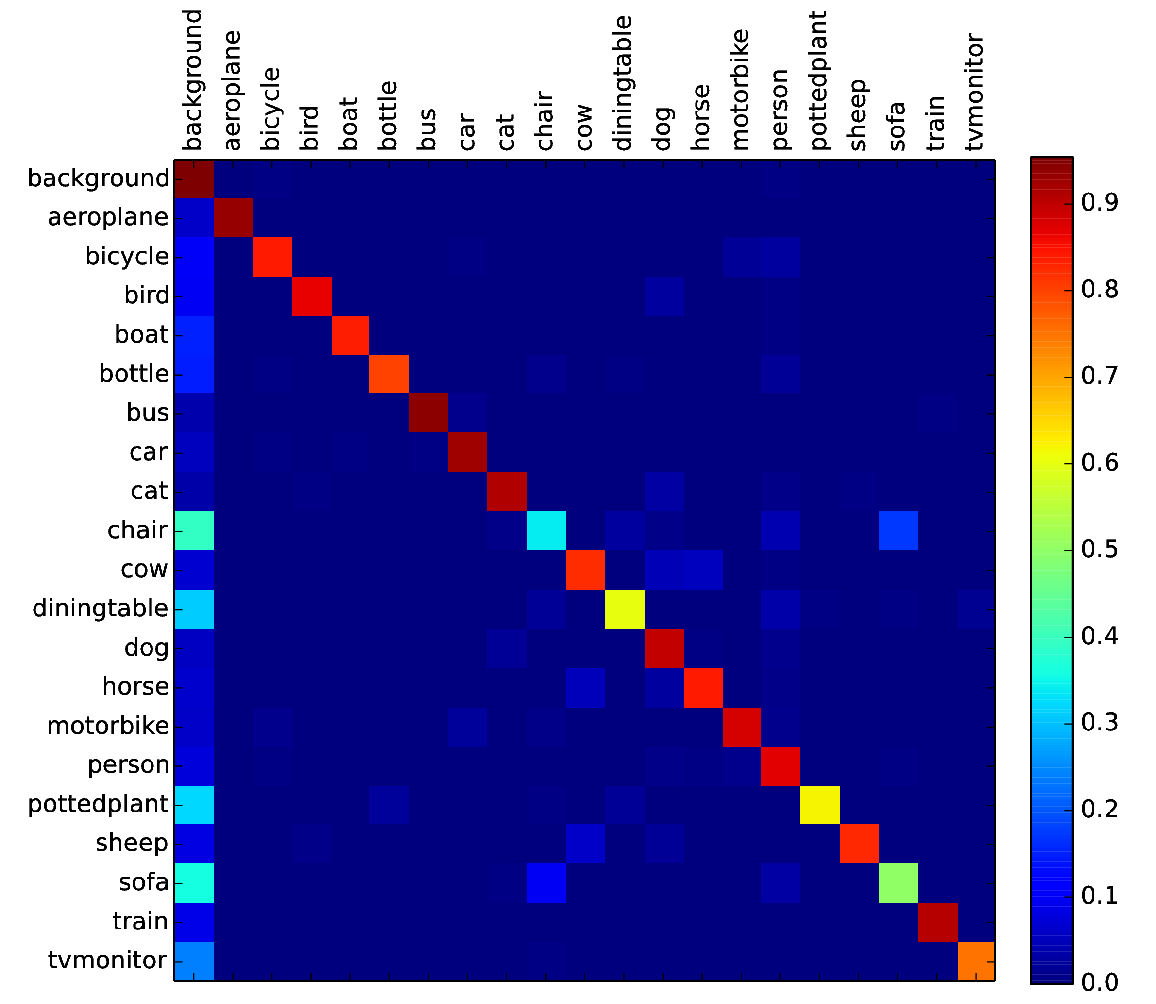
\includegraphics[width=0.5\textwidth]{image/result/confusion.pdf}
% 	\caption{镶嵌在文中的图像}
% 	\captionce[图注]{这是测试图注。}{A testing figure legend.}\label{fig:test}
% 	\label{fig:confusion}
% \end{figure}

\end{document}
